%*******************************************************************************
% Title: Performance Modeling of Computer Systems and Networks
%
% Conference: Computer Science Lectures 2017
%
% Authors: Giacomo Marciani <gmarciani@ieee.org>
%
% Institution: Department of Civil Engineering and Computer Science Engineering,
% 			   University of Rome Tor Vergata, Italy
%
% Style: ACM Large VERSION 1.7
%*******************************************************************************

\documentclass[prodmode,gmlecture]{acmlarge}

%*******************************************************************************
% Packages
%*******************************************************************************
\usepackage[utf8]{inputenc}
\usepackage{amsmath}
\usepackage{lipsum}
\usepackage{xr}
\usepackage{hyperref}
\usepackage{cleveref}

%*******************************************************************************
% Details
%*******************************************************************************
\acmVolume{2}
\acmNumber{1}
\acmArticle{1}
\articleSeq{1}
\acmMonth{9}
\acmYear{2016}

\issn{1234-56789}
\doi{0000001.0000001}

%*******************************************************************************
% Copyright
%*******************************************************************************
\setcopyright{rightsretained}

%*******************************************************************************
% Algorithm
%*******************************************************************************
\usepackage[ruled]{algorithm2e}
\SetAlFnt{\algofont}
\SetAlCapFnt{\algofont}
\SetAlCapNameFnt{\algofont}
\SetAlCapHSkip{0pt}
\IncMargin{-\parindent}
\renewcommand{\algorithmcfname}{ALGORITHM}

%*******************************************************************************
% Notations
%*******************************************************************************
\newcommand{\probability}[1]{
	\mathbf{P}[#1]
}
\newcommand{\expected}[1]{
	\mathbf{E}[#1]
}
\newcommand{\variance}[1]{
	\mathbf{Var}[#1]
}

%*******************************************************************************
% Numbering
%*******************************************************************************
\numberwithin{equation}{section}

%*******************************************************************************
% References
%*******************************************************************************
\crefname{lem}{lemma}{lemmata}
\Crefname{cor}{Corollary}{Corollaries}
\externaldocument{sec/queueing-theory}
\externaldocument{sec/operational-laws}
\externaldocument{sec/asymptotic-analysis}
\externaldocument{sec/modification-analysis}
\externaldocument{sec/exponential-distribution}
\externaldocument{sec/poisson-processes}
\externaldocument{sec/markov-chains}
\externaldocument{sec/server-farms}
\externaldocument{sec/m-m-1-queues}
\externaldocument{sec/m-m-m-m-queues}
\externaldocument{sec/m-m-m-queues}
\externaldocument{sec/m-m-inf-queues}
\externaldocument{sec/m-g-1-queues}
\externaldocument{sec/m-m-1-ps-queues}
\externaldocument{sec/capacity-provisioning}
\externaldocument{sec/burke-theorem}
\externaldocument{sec/networks-of-queues}
\externaldocument{sec/open-jackson-networks}
\externaldocument{sec/closed-jackson-networks}
\externaldocument{sec/mean-value-analysis}
\externaldocument{sec/task-assignment-policies-server-farms}
\externaldocument{sec/scheduling-m-g-1}
\externaldocument{sec/scheduling-non-preemptive-non-size-based}
\externaldocument{sec/scheduling-preemptive-non-size-based}
\externaldocument{sec/scheduling-non-preemptive-size-based}
\externaldocument{sec/scheduling-preemptive-size-based}
\externaldocument{sec/random-variables-simulation}
\externaldocument{sec/formulary-probability}
\externaldocument{sec/formulary-queueing-theory}
\externaldocument{sec/tips-tricks}
\externaldocument{sec/related-readings}

%*******************************************************************************
% Title and Authors
%*******************************************************************************
\markboth{G. Marciani}{Performance Modeling of Computer Systems and Networks}
\title{Performance Modeling of Computer Systems and Networks}
\author{GIACOMO MARCIANI \affil{University of Rome Tor Vergata}}

%*******************************************************************************
% Content
%*******************************************************************************

% From mitthesis package
% Version: 1.01, 2023/06/19
% Documentation: https://ctan.org/pkg/mitthesis
%
% The abstract environment creates all the required headers and footnote. 
% You only need to add the text of the abstract itself.
%
% Approximately 500 words or less; try not to use formulas or special characters
% If you don't want an initial indentation, do \noindent at the start of the abstract

The developments of the ``kinetic theory'' of gases made within the last ten years have enabled it to account satisfactorily for many of the laws of gases. The mathematical deductions of Clausius, Maxwell and others, based upon the hypothesis of a gas composed of molecules acting upon each other at impact like perfectly elastic spheres, have furnished expressions for the laws of its elasticity, viscosity, conductivity for heat, diffusive power and other properties. For some of these laws we have experimental data of value in testing the validity of these deductions and assumptions. Next to the elasticity, perhaps the phenomena of the viscosity of gases are best adapted to investigation.\footnote{Text from Holman (1876): \doi{10.2307/25138434}.}  

% http://dl.acm.org/ccs.cfm

\begin{CCSXML}
    <ccs2012>
    <concept>
        <concept_id>10002944.10011122.10002945</concept_id>
        <concept_desc>General and reference~Surveys and overviews</concept_desc>
        <concept_significance>500</concept_significance>
    </concept>
    <concept>
        <concept_id>10002978</concept_id>
        <concept_desc>Security and privacy</concept_desc>
        <concept_significance>500</concept_significance>
    </concept>
    <concept>
        <concept_id>10002978.10003022</concept_id>
        <concept_desc>Security and privacy~Software and application security</concept_desc>
        <concept_significance>500</concept_significance>
    </concept>
    </ccs2012>
\end{CCSXML}

\ccsdesc[500]{General and reference~Surveys and overviews}
\ccsdesc[500]{Security and privacy~Software and application security}

\keywords{computer security; botnet}


\acmformat{Giacomo Marciani. 2016. Performance Modeling of Computer Systems and Networks.}

\begin{document}

\begin{bottomstuff}
	This work is supported by the Department of Civil Engineering and Computer Science
	Engineering, University of Rome Tor Vergata, Italy.\\
	Author's address: G. Marciani, Via del Politecnico 1, Rome, RM 00133, Italy;
	email: gmarciani@ieee.org.
\end{bottomstuff}

\maketitle

\section{Queueing Theory}
\label{sec:Queueing-Theory}

The queueing theory is built on the stochastic modeling and analysis, which represents service demands and interarrivals as random variables.
It is the theory behind what makes queues appear and how to make them go away.
It is the study of queueing behavior in systems and networks.

Queueing theory applies anywhere that queues come up. It is also at the heart of any computer system.

Queueing theory has its origins in research by Agner Krarup Erlang when he created models to describe the Copenhagen telephone exchange.

Queues results from variability in service time and/or interarrival time distribution.

A major reason why computer scientists are so slow to adopt queueing theory is that standard assumptions often do not fit. In some cases they are very far from reality: for example, in the case of high variability and correlations. However there are often ways to work around these assumptions.

The goals of a queueing theorist is \textit{predicting} the system performance and \textit{designing} it to improve performance.

There are many questions in computer systems design that lend themselves to a queueing-theoretic solution (e.g., power management, priority scheduling, and so on).
However, there are  lots of problems that we can at best only analyze approximately (e.g., mean response time for M/G/k queue). Typically, approximations are very poor when jobs size variability gets high \cite{gupta2010inapproximability}.




\subsection{Queue Metrics}
\label{sec:Queue-Metrics}

A queue node is described by the following parameters and performance metrics:

\begin{description}
	\item [Service Order] The scheduling discipline.
	
	\item [Average Arrival Rate]  ($\lambda$) The rate at which jobs arrive to the node.
	
	\item [Interarrival Time] ($\tau$) The time between successive job arrivals.
	
	\item [Mean Interarrival Time] ($\expected{\tau}=\frac{1}{\lambda}$) The average time between successive job arrivals.
	
	\item [Service Requirement, Size] ($S$) The time taken by a job to run on server.
	
	\item [Average Service Rate] ($\mu$) The rate at which jobs are served by the server.
	
	\item [Mean Service Time] ($\expected{S}=\frac{1}{\mu}$) The average time required to serve a job.
	
	\item [Waiting Time, Delay] ($T_{Q}$) The time that the job spends in the queue.
	
	\item [Response Time, Turnaround Time] ($T$) The time during which the job is in the node. Thus $T=T_{departure}-T_{arrival}$. Note that $\expected{T}=\expected{T_{Q}}+\expected{S}$.
	
	\item [Number of System Jobs] ($N$) The number of jobs in the queue plus the ones being served.
	
	\item [Number of Queued Jobs] ($N_{Q}$) The number of jobs in the queue.
	
	\item [Utilization] ($\varrho$) The fraction of time the server is busy, the probability of the server to be busy, the mean number of jobs in that node.
	
	\item [Throughput] ($X$) The rate of completions at server.
\end{description}




\subsection{Kendall notation}
A queue node il classified using the Kendall notation \cite{kendall1953stochastic}.

\begin{equation}
A/S/m/c/N/D
\end{equation} 

where 

\begin{description}
	\item [A] the arrival process, the value indicates the probability distribution of inter-arrival times.
	
	\item [S] the service process, the value indicates the probability distribution of service times.
	
	\item [A] the number of servers.
	
	\item [c] the capacity of the system (that is, the number of servers plus the buffer size).
	
	\item [N] the size of the population, that is the total number of jobs.
	
	\item [D] the scheduling discipline.
\end{description}

The arrival process \textit{A} and service process \textit{S} could be equal to 

\begin{description}
	\item [$M$] Exponential distribution.
	
	\item [$D$] Deterministic distribution.
	
	\item [$E_{n}$] Erlang distribution of order $n$.
	
	\item [$H_{n}$] Hyper-exponential distribution of order $n$.
	
	\item [$G$] Generic distribution of independent variables.
\end{description}

The scheduling discipline \textit{D} could be equal to 

\begin{description}
	\item [$FCFS (FIFO)$] first come, first served.
	
	\item [$LCFS (LIFO)$] last come, first served.
	
	\item [$RO$] random order.
	
	\item [$RR$] round robin.
	
	\item [$PS$] processor sharing.
	
	\item [$P$] custom priority.
\end{description}

When the final three parameters are not specified (e.g. M/M/1 queue), it is assumed $K=\infty$, $N=\infty$ and $D=FIFO$.




\subsection{Classification of Queueing Networks}
\label{sec:Classification-Queueing-Networks}

Queueing networks can be classified into two categories:

\begin{description}
	\item [Open Networks] They have external arrivals and departures. In such systems, $X=\lambda$
	
	\item [Closed Networks] They have no external arrivals or departures. In such systems, $X=\mu$. The number of jobs in the system is fixed to $N$, and it is called \textit{load} or \textit{multiprogramming level (MPL)}. $\expected{T}=\expected{T_{R}}+\expected{Z}$. Closed networks can be classified in two categories:
	
	\begin{description}
		\item [Interactive Networks] There are $N$ \textit{terminals} which submit jobs to a network of queues, called \textit{central subsystem}. After submission, a terminal waits for job completion, then sleeps for a think-time $Z$, then can submit again. Thus, a terminal oscillates between a submission-state and a think-state. The goal is to limit the rise of $\expected{T_{R}}$ with $N$.
		
		\item [Batch Networks] They are interactive networks with no think-time ($Z=0$). The goal is to obtain high throughput.
	\end{description}		
	
\end{description}

%\begin{figure}[tp]
%\label{fig:Open-Network-Sample}
%	\centering
%	
\includegraphics{fig/Open-Network-Sample}
%	\caption{An Open network.}
%\end{figure}

%\begin{figure}[tp]
%\label{fig:Interactive-Network-Sample}
%	\centering
%	
\includegraphics{fig/Interactive-Network-Sample}
%	\caption{An Interactive network.}
%\end{figure}

%\begin{figure}[tp]
%\label{fig:Batch-Network-Sample}
%	\centering
%	
\includegraphics{fig/Batch-Network-Sample}
%		\caption{A Batch network.}
%\end{figure}

\cite{schroeder2006open} proposed the notion of \textit{partly-open networks}. Here terminals arrive from outside as in open networks, but make request as in closed ones.




\subsection{Utilization}
\label{sec:Utilization}

The utilization of a queue node is the fraction of time the node is busy, the probability that it is busy, and the mean number of jobs in that node.

\begin{theorem}[Utilization Law]
\label{thm:Utilization-Law}

	For every stable queue node, we have that:
	
	\begin{equation}
	\label{eqn:Utilization-Law}
	\varrho = \frac{\lambda}{\mu} = X \cdot \mathbf{E}[S]
	\end{equation}
	
	\begin{proof}
		Let us consider the definition of throughput ($X=\frac{C}{\tau}$) and utilization ($\varrho=\frac{B}{\tau}$). We have that
		
		\begin{equation*}
			X = \frac{C}{\tau} = \frac{C}{B} \cdot \frac{B}{\tau} = \frac{C}{B} \cdot \varrho
		\end{equation*}
		
		Since $\frac{B}{C}=\expected{S}$ and $\frac{C}{B}=\mu$, we have that
		
		\begin{equation*}
			X = \mu \cdot \varrho \equiv \frac{\varrho}{\expected{S}} \Rightarrow \varrho = X \cdot \expected{S}
		\end{equation*}
	\end{proof}
\end{theorem}




\subsection{Stability}
\label{sec:Stability}

The stability condition guarantees that the queue cannot grow unbounded.

\begin{theorem}
\label{thm:Stability}
	A queue node is stable if and only if \footnote{The condition is necessary, but there are more complex networks (not examined here) where it is not sufficient \cite{bramson2008stability}.} 
	
	\begin{equation}
	\label{eqn:Stability}
	\lambda < \mu
	\end{equation}
	
	\begin{proof}
		Let's prove that if $\lambda > \mu$ then the queue would grow to infinity over time.		
		Given a time $t$, the number of system jobs $N(t)$, the number of arriving jobs $A(t)$ and the number of departing jobs $D(t)$, we have that
		
		\begin{equation*}
		\expected{N(t)}=\expected{A(t)}-\expected{D(t)} \geq t(\lambda - \mu)
		\end{equation*}
		
		where the inequality holds because the server is not always busy, then the departures at time $t$ are less than $\mu t$. 
		At the end, we have that
		
		\begin{equation*}
		\lambda > \mu \Rightarrow \lim_{t \to \infty} \expected{N(t)} = \infty
		\end{equation*}
	\end{proof}
\end{theorem}
\section{Operational Laws}
\label{sec:Operational-Laws}

Operational laws are laws that hold for any open/closed system \footnote{they often are most powerful when applied to closed ones.} or part of it.
They are distribution independent and depends only on mean quantities.
Operational laws can be put together to prove asymptotic bounds on closed networks behavior.
These asymptotic bounds are useful to answer what-if questions.
They are fundamental for the modification analysis.

In the following sections, we present the following operational laws: 
\textit{Little's Law},
\textit{Utilization Law},
\textit{Forced Flow Law}, and 
\textit{Bottleneck Law}.




\subsection{Little's Law}
\label{sec:Little-Law}

The Little's Law \cite{little1961proof} is the most important operational law. It relates mean number of system jobs to the mean response time.

\begin{theorem}[Little's Law for open systems]
\label{thm:Little-Law-Open-Systems}	
	For any ergodic open system, we have that
	
	\begin{equation}
	\label{eqn:Little-Law-Open-Systems}
	\expected{N} = \lambda \cdot \expected{T}
	\end{equation}
	
	where $\expected{N}$ is the expected number of jobs in the system, $\lambda$ is the average arrival rate into the system, and $\expected{T}$ is the mean time jobs spend in the system.
\end{theorem}

\begin{theorem}[Little's Law for closed systems]
\label{thm:Little-Law-Closed-Systems}	
	For any ergodic closed system, we have that
	
	\begin{equation}
	\label{eqn:Little-Law-Closed-Systems}
	N = X \cdot \expected{T}
	\end{equation}
	
	where $N$ is the multiprogramming level, $X$ is the throughput, and $\expected{T}$ is the mean time jobs spend in the system.
\end{theorem}

It is important to note that Little's Law makes no assumption on arrival process, service process, network topology or anything else. It only requires the system to be in steady state with finite $\expected{N}$ and $\expected{T}$.

The Little's Law holds for higher moments only under very restrictive conditions (e.g. it requires FCFS \cite{bertsimas1995distributional,brumelle1972generalization}).

The Little's Law take into account the \textit{effective arrival rate}. Be aware to consider the three quantities in Little's Law on the same request flow.

The following is an alternative expression of the Little's Law for closed systems.

\begin{corollary}
\label{cor:Response-Time-Law-Closed-Systems}
	
	For every ergodic closed system, we have that
	
	\begin{equation}
	\label{eqn:Response-Time-Law-Closed-Systems}
	\expected{R} = \frac{N}{X} - \expected{Z}
	\end{equation}
	
	where 
	$\expected{R}$ is the expected response time,
	$N$ is the multiprogramming level,
	$X$ is the system throughput, and
	$\expected{Z}$ is the expected think time.
	
	\begin{proof}
		The corollary directly follows from the Little's Law.
		\begin{equation*}
		\begin{split}
		N & = X \cdot \expected{T} \\
		& = X \cdot (\expected{R} + \expected{Z}) 
		\end{split}
		\end{equation*}
		So we have
		\begin{equation*}
		\expected{R} = \frac{N}{X} - \expected{Z}
		\end{equation*}
	\end{proof}
\end{corollary}




\subsection{Utilization-Law}
\label{sec:Utilization-Law}

\begin{theorem}[Utilization Law]
\label{thm:Utilization-Law-2}	
	For every stable queue node we have that
	
	\begin{equation}
	\varrho = \frac{\lambda}{\mu}
	\end{equation}
	
	where $\varrho$ is the long-run fraction of time that the server is busy.
	
	\begin{proof}
		Let us consider only the server of the queue node, without the associated queue. The number of jobs in the node is 1 with probability $\varrho$ and 0 with probability $(1-\varrho)$. Hence the the expected number of jobs in the node is $\varrho$.
		So, applying Little's Law, we have
		\begin{equation*}
			\begin{split}
			\varrho & = \expected{N} \\
					& = \lambda \cdot \expected{T} \\
					& = \lambda \cdot \expected{S} \\
					& = \lambda \cdot \frac{1}{\mu}
			\end{split}
		\end{equation*}
	\end{proof}
\end{theorem}

Notice that

\begin{equation}
\varrho_{i} = \probability{server \; i \; busy} = \expected{requests \; to \; server \; i}
\end{equation}
That is, the utilization is the probability to have the server busy and the expected number of requests being served.




\subsection{Forced Flow Law}
\label{sec:Forced-Flow-Law}

\begin{theorem}[Forced Flow Law]
\label{thm:Forced-Flow-Law}	
	For every stable network of queues, we have that
	
	\begin{equation}
	\label{eqn-Forced-Flow-Law}
	X_{i} = \expected{V_{i}} \cdot X
	\end{equation}
	
	where 
	$X$ is the system throughput,
	$X_{i}$ is the throughput at the \textit{i}-th server, and
	$V_{i}$ is the visit ratio for the \textit{i}-th server, that is the number of visits per job to the \textit{i}-th server.
	
	\begin{proof}
		Let us first consider a intuitive demonstration.
		For every system completion, there are on average $\expected{V_{i}}$ completions at the \textit{i}-th server. Hence the rate of completions at the \textit{i}-th server is $\expected{V_{i}}$ times the rate of system completions.
		
		Let us now consider a more formal demonstration.
		Let $C(t)$ denote the system completions during time $t$, $C_{i}(t)$ denote the completions at the \textit{i}-th server during time $t$, and $V_{i}^{(i)}$ denote the number of visits the the \textit{j}-th job makes to the \textit{i}-th server. Then,
		\begin{equation*}
			\begin{split}
				C_{i}(t) & = \sum_{j \in C(t))}V_{i}^{(j)} \\
				\frac{C_{i}(t)}{t} & = \frac{\sum_{j \in C(t))}V_{i}^{(j)} }{C(t)} \cdot \frac{C(t)}{t} \\
				\lim_{t \to \infty} \frac{C_{i}(t)}{t} & = \lim_{t \to \infty} \frac{\sum_{j \in C(t))}V_{i}^{(j)} }{C(t)} \cdot \lim_{t \to \infty} \frac{C(t)}{t} \\
				X_{i} & = \expected{V_{i}} \cdot X
			\end{split}
		\end{equation*}
	\end{proof}
\end{theorem}




\subsection{Bottleneck Law}
\label{sec:Bottleneck-Law}

We define $D_{i}$ to be the total service demand on the \textit{i}-th server

\begin{equation}
D_{i} = \sum_{j=1}^{V_{i}}S_{i}^{(j)}
\end{equation}

Since $V_{i}$ and $S_{i}^{(j)}$ are independent, we have that

\begin{equation}
\label{eqn:Service-Demand}
\expected{D_{i}} = \expected{V_{i}} \cdot \expected{S_{i}}
\end{equation}

In practice, we measure $\expected{D_{i}}$ as follows

\begin{equation}
\expected{D_{i}} = \frac{B_{i}}{C} 
\end{equation}

where
$B_{i}$ is the busy time for the \textit{i}-th server, and
$C$ is the system completions.

Let $m$ be the number of servers in our system. Let

\begin{equation}
\label{eqn:Total-Demand}
D = \sum_{i=1}^{m}\expected{D_{i}}
\end{equation}

and

\begin{equation}
\label{eqn:Maximum-Demand}
D_{max} = \max\{\expected{D_{i}}\}
\end{equation}

Previous definitions will be useful when discussing \textit{Bottleneck Law}, \textit{asymptotic bounds} and \textit{modification analysis}.

\begin{theorem}[Bottleneck Law]
\label{thm:Bottleneck-Law}	
	For every stable network of queues, we have that
	
	\begin{equation}
	\label{eqn:Bottleneck-Law}
	\varrho_{i} = X \cdot \expected{D_{i}}
	\end{equation}
	
	where 
	$\varrho_{i}$ is the utilization of the \textit{i}-th server, 
	$X$ is the system throughput, and
	$\expected{D_{i}}$ is the expected service demand on the \textit{i}-th server for all visits of a single job.
	
	\begin{proof}
		Let us first consider an intuitive demonstration.
		Let $X$ denote the job/sec arrival rate to the whole system and let each arrival contribute $\expected{D_{i}}$ seconds of work for the \textit{i}-th server. We have that the \textit{i}-th server is busy for $X \cdot \expected{D_{i}}$ seconds out of every second.
		Thus $X \cdot \expected{D_{i}}$ represents the utilization of the \textit{i}-th server.
		
		Let us now consider a more formal demonstration.
		Let us consider 
		the Utilization Law ($\varrho = X \cdot \expected{S}$),
		the Forced Flow Law ($X_{i} = \expected{V_{i}} \cdot X$), and
		the demand definition ($D_{i} = \sum_{j=1}^{V_{i}}S_{i}^{(j)} \Rightarrow \expected{D_{i}} = \expected{V_{i}} \cdot \expected{S_{i}}$).
		We have that
		\begin{equation*}
			\begin{split}
				\varrho_{i} & = X_{i} \cdot \expected{S_{i}} \\
							& = X \cdot \expected{V_{i}} \cdot \expected{S_{i}} \\
							& = X \cdot \expected{D_{i}}
			\end{split}
		\end{equation*}
	\end{proof}
\end{theorem}
\section{Asymptotic Analysis for Closed Systems}
\label{sec:Asymptotic-Analysis-Closed-Systems}

\begin{theorem}[Asymptotic Bounds for Closed Systems]
	\label{thm:Asymptotic-Bounds-Closed-Systems}
	For any closed system with load $N$, we have that
	
	\begin{equation}
	\label{eqn:Asymptotic-Bounds-Closed-Systems}
	\begin{split}
	X & \leq \min \Big\{ \frac{N}{D + \expected{Z}} , \frac{1}{D_{max}} \Big\} \\
	\expected{R} & \geq \max\{D , N \cdot D_{max} - \expected{Z} \}
	\end{split}
	\end{equation}
	
	where the first term in each clause is an asymptote for small $N$, and the second one for large $N$.
	
	\begin{proof}
		See \cite{harchol2013performance} for a formal demonstration.
	\end{proof}
\end{theorem}

It is possible to get even tighter bounds by using the \textit{Balanced Bounds technique}, described in \cite{lazowska1984quantitative}.

The lower and the upper bound intercept in 
\begin{equation}
\label{eqn:Asymptotic-Bounds-Closed-Systems-Interception}
N^{*} = \frac{D + \expected{Z}}{D_{max}}
\end{equation}
That is the point beyond which there must be some queueing in the system, because $\expected{R} > D$.

If $N > N^{*}$, performance can be improved ($X$ increased and $\expected{R}$ decreased) only decreasing $D_{max}$.

If $N >> N^{*}$, decreasing some $D_{i} < D_{max}$ have no effect.
If $N << N^{*}$, decreasing some $D_{i} < D_{max}$ have little effect.

In a batch system ($Z=0$), $N^{*}$ decreases, meaning that the domination of $D_{max}$ occurs with smaller load.

The bottleneck server is the server with demand $D_{max}$. It is the key limiting factor to performance improvement. Thus, the first step in improving performance is to identify the bottleneck server.

The asymptotic bounds hold for open systems only if $\lambda . X \rightarrow \frac{1}{D_{max}}$.
\section{Modification Analysis}
\label{sec:Modification-Analysis}

The modification analysis is the procedure to evaluate modifications with respect to the achievable performance improvements. The analysis leverages the asymptotic bounds stated in \Cref{sec:Asymptotic-Bounds}.

The modification analysis is computationally feasible, does not rely on any assumption about arrival process, service process or scheduling policy. It is a powerful tool because bounds behavior is what we need when evaluating performance improvements.
\section{Exponential Distribution}
\label{sec:Exponential-Distribution}

The arrival and service processes can follow whichever probabilistic distribution. Most often, inter-arrival and service times follow the exponential distribution, because of its wide applicability and mathematical tractability.
The Exponential distribution is the continuous counterpart of the Geometric distribution. The Geometric distribution models the number of attempts until the first success, whereas the Exponential distribution models the time until the first success.

\begin{definition}[Exponential Distribution]
\label{def:Exponential-Distribution}	
	A random variable $X$ is Exponentially distributed with rate\footnote{if $X \sim Exp(\lambda)$, $\lambda$ is called \textit{rate} because $\expected{X}=\frac{1}{\lambda}$.} $\lambda$ ($X \sim Exp(\lambda)$) if $X$ has the following probability density function:
	
	\begin{equation}
	\label{eqn:Exponential-PDF}
	f(x) = \left\{\begin{matrix}
		\lambda e^{-\lambda x} & x \geq 0\\ 
		0 & x \leq 0
	\end{matrix}\right.
	\end{equation}
\end{definition}

The p.d.f of $X \sim Exp(\lambda)$ is shown in \Cref{fig:Exponential-PDF}.

\begin{figure}[tp]
\label{fig:Exponential-PDF}	
	\centering
	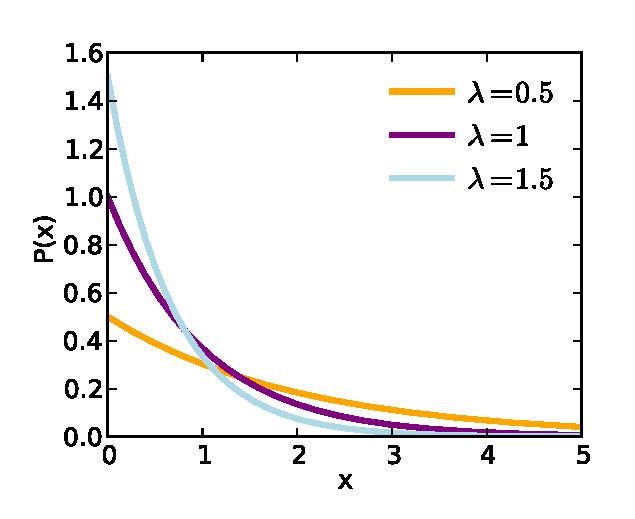
\includegraphics{fig/exponential-pdf}
	\caption{Exponential p.d.f.}
\end{figure}

From the \Cref{def:Exponential-Distribution} follows that the cumulative distribution function of $X \sim Exp(\lambda)$ is

\begin{equation}
\label{eqn:Exponential-CDF}
\begin{aligned}
	F(x) = \int_{- \infty}^{x} \partial y = 
	\left\{\begin{matrix}
	1 - e^{-\lambda x} & x \geq 0\\ 
	0 & x \leq 0
	\end{matrix}\right.
\end{aligned}
\end{equation}

The Exponential distribution has moments

\begin{equation}
\label{eqn:Exponential-Mean}
\expected{X} = \int_{- \infty}^{\infty} xf(x) \partial x = \frac{1}{\lambda}
\end{equation}

\begin{equation}
\label{eqn:Exponential-Moment-2}
\expected{X^{2}} = \int_{- \infty}^{\infty} x^{2}f(x) \partial x = \frac{2}{\lambda^{2}}
\end{equation}

and variance

\begin{equation}
\label{eqn:Exponential-Variance}
	\variance{X} = \expected{X^{2}} - \expected{X}^{2} = \frac{1}{\lambda^{2}}
\end{equation}

The Exponential distribution is so convenient because it is memoryless. In particular, the Exponential distribution is the only continuous memoryless distribution.

\begin{theorem}[Exponential Memoryless]
\label{thm:Exponential-Memoryless}

	A random variable $X \sim Exp(\lambda)$ is memoryless.
	
	\begin{proof}
		\begin{equation*}
		\probability{X > s+t | X > s}=\frac{X > s+t}{X > s}=\frac{e^{- \lambda (s+t)}}{e^{- \lambda s}}=e^{- \lambda t}=\probability{X > t}
		\end{equation*}
	\end{proof}
\end{theorem}

The Exponential distribution is memoryless and with constant failure rate. It exposes also the following useful properties.

\begin{theorem}[Precedency of Exponentials]
\label{thm:Exponential-Precedency}
	Given independent $X_{1} \sim Exp(\lambda_{1})$ and $X_{2} \sim Exp(\lambda_{2})$, we have that
	
	\begin{equation}
	\label{eqn:Exponential-Precedency}
	\probability{X_{1} < X_{2}} = \frac{\lambda_{1}}{\lambda_{1} + \lambda_{2}}
	\end{equation}
\end{theorem}

\begin{theorem}[Minimum Exponentials]
\label{thm:Exponential-Minimum}
	Given independent $X_{1} \sim Exp(\lambda_{1})$ and $X_{2} \sim Exp(\lambda_{2})$, we have that
	
	\begin{equation}
	\label{eqn:Exponential-Minimum}
	\min(X_{1},X_{2}) \sim Exp(\lambda_{1} + \lambda_{2})
	\end{equation}
\end{theorem}
\section{Poisson Processes}
\label{sec:Poisson-Processes}

The Poisson process is the most widely used model for arrivals into a system because it is often a realistic representation of natural models and, since it exposes the Markovian property, it is analytically tractable.
It greatly models natural process where we observe aggregation of large number of independent entities \footnote{This is true thanks to the Limiting Theorem \cite{ross2014introduction}}.

The Poisson distribution is a discrete probability distribution that expresses the probability of a given number of events occurring in a fixed interval of time and/or space if these events occur with a known average rate and independently of the time since the last event. If inter-arrival times are Exponentially distributed, then the number of arrivals within a given time is Poisson distributed.

\begin{definition}[Poisson Distribution]
\label{def:Poisson-Distribution}
	A random variable $N(t)$ is Poisson distributed with rate\footnote{if $N(t) \sim Poisson(\lambda)$, $\lambda$ is called \textit{rate} because $\expected{N(t)}=\lambda t$.} $\lambda$ ($N(t) \sim Poisson(\lambda)$) if $N(t)$ has the following probability mass function:
	
	\begin{equation}
	\label{eqn:Poisson-PMF}
	f(k,t) = \frac{(\lambda t)^{k} e^{-\lambda t}}{k!}
	\end{equation}
\end{definition}

The p.d.f of $X \sim Poisson(\lambda)$ is shown in \Cref{fig:poisson-pdf}.

\begin{figure}[tp]
\label{fig:Poisson-PMF}	
	\centering
	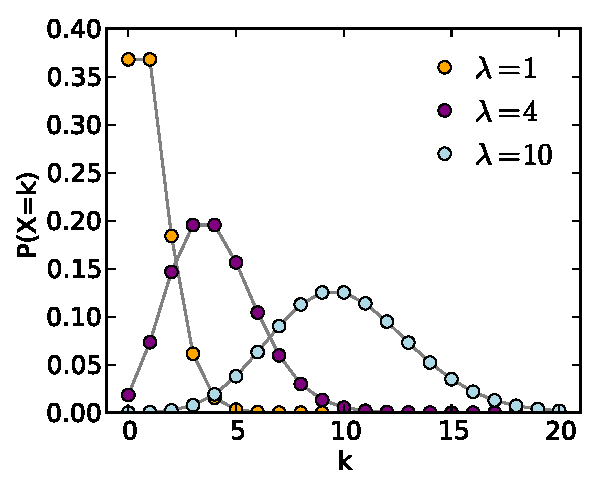
\includegraphics{fig/poisson-pdf}
	\caption{Poisson p.m.f.}
\end{figure}

From the \Cref{def:Poisson-Distribution} follows that the cumulative distribution function of $N(t) \sim Poisson(\lambda)$ is 

\begin{equation}
\label{eqn:Poisson-CDF}
F(k,t) = \sum_{x=0}^{t} f(k,x)
\end{equation}

The Poisson distribution has mean

\begin{equation}
\label{eqn:Poisson-Mean}
\expected{N(t)} = \lambda t
\end{equation}

and variance

\begin{equation}
\label{eqn:Poisson-Variance}
\variance{N(t)} = \lambda t
\end{equation}

\begin{definition}[Poisson Process]
\label{def:poisson-process-statistical}
	A Poisson process with rate $\lambda$ is a sequence of events such that
	(i) $N(0)=0$,
	(ii) it has independent increments,
	(iii) $\probability{N(s+t)-N(s) = n} \sim Poisson(\lambda t)$
\end{definition}

Notice that point (iii) in \Cref{def:poisson-process-statistical} implies stationary increments. 
Furthermore, the assumption of independent and stationary increments implies that, at any point in time, the process statistically restarts itself; that is, the process from any point onward is independent of all previously occurred (independent increments) and has the same distribution of the original process (stationary increments).

\begin{definition}[Poisson Process]
\label{def:poisson-process-practical}
	A Poisson process with rate $\lambda$ is a sequence of events such that
	(i) the interarrival times are Exponential r.v. with rate $\lambda$, and 
	(ii) $N(0)=0$.
\end{definition}

A Poisson process has stationary and independent increments.

Here are some useful properties of the Poisson distribution.

\begin{theorem}[Poisson Merging]
\label{thm:Poisson-Merging}	
	Given two independent Poisson process with rate $\lambda_{1}$ and $\lambda_{2}$, the merged process is a Poisson process with rate $(\lambda_{1} + \lambda_{2})$.
\end{theorem}

\begin{theorem}[Poisson Splitting]
\label{thm:Poisson-Splitting}	
	Given a Poisson process with rate $\lambda$, whose events are partitioned in class-A with probability $p$ and class-B with probability $(1-p)$, the class-A process is a Poisson process with rate $p \lambda$ and the class-B process is a Poisson process with rate $(1-p) \lambda$, and these processes are independent.
\end{theorem}

\begin{theorem}[Poisson Uniformity - Single Event]
\label{thm:Poisson-Uniformity-Single-Event}	
	Given that one event of a Poisson process has occurred by time $t$, that event is equally likely to have occurred anywhere in $[0,t]$. 
\end{theorem}

\begin{theorem}[Poisson Uniformity - Multiple Events]
\label{thm:Poisson-Uniformity-Multiple-Events}	
	If $k$ events of a Poisson process occur by time $t$, then the $k$ events are distributed independently and uniformly in $[0,t]$. 
\end{theorem}
\section{Markov Chains}
\label{sec:markov-chains}

\begin{definition}[Markovian Property]
\label{def:markovian-property}
	The Markovian property states that the conditional distribution of any future state $X_{n+1}$, given past states $X_{0},X_{1},...,X_{n-1}$, and given the present state $X_{n}$, is independent of past states and depends only on the present state.
\end{definition}

\begin{definition}[Discrete-Time Markov Chain]
\label{def:discrete-time-markov-chain}

	A Discrete-Time Markov Chain (DTMC) is a stochastic process $\{X_{n \in \natural}\}$, where $X_{n}$ denotes the state at time $n$ and such that
	
	\begin{equation}
	\label{eqn:discrete-time-markov-chain}
		\begin{split}	
			\probability{X_{n+1} = j | X_{n} = i,X_{n-1} = i_{n}-1,...,X_{0} = i_{0}}
			& = \probability{X_{n+1} = j | X_{n} = i} \\
			& = P_{i,j} \\
			& \forall n \geq 0, \forall i,j, \forall i_{0},...,i_{n-1}
		\end{split}		
	\end{equation}
	
	where $P_{i,j}$ is independent of time and past history.
\end{definition}

\begin{definition}[Continuous-Time Markov Chain]
\label{def:continuous-time-markov-chain}
	
	A Continuous-Time Markov Chain (CTMC) is a stochastic process $\{X(t),t \in \Re^{+}\}$, where $X_{n}$ denotes the state at time $n$ and such that
	
	\begin{equation}
	\label{eqn:continuous-time-markov-chain}
		\begin{split}	
			\probability{X(s+t) = j | X(s) = i,X(u) = x(u)} 
			& = \probability{X(s+t) = j | X(s) = i} \\
			& = \probability{X(t) = j | X(0) = i} \\
			& = P_{i,j}(t) \\
			& \forall s,t \geq 0, \forall i,j,x(u) 
		\end{split}		
	\end{equation}
	
	where $P_{i,j}$ is independent of time and past history.
\end{definition}

Alternatively

\begin{definition}[Continuous-Time Markov Chain 2]
	\label{def:continuous-time-markov-chain-2}
	
	A Continuous-Time Markov Chain (CTMC) is a stochastic process with the property that every time it enters state $i$, the following hold:
	
	\begin{enumerate}
		\item The amount of time the process spends in state $i$ is a r.v. $X \sim Exp(\lambda)$.
		
		\item The probability $p_{i,j}$ to transit from state $i$ to state $j$ is independent of the time spent in state $i$.
	\end{enumerate}
\end{definition}

\begin{definition}[Transition Probability Matrix]
\label{def:transition-probability-matrix}
	
	The transition probability matrix associated with any Markov chain is a matrix, whose $(i,j)$-th entry $P_{i,j}$ is the probability of moving in the next transition from state $i$ to state $j$.
\end{definition}

By definition, we have that 

\begin{equation*}
\sum_{j} P_{i,j} = 1 \quad \forall i
\end{equation*}

A queue network that exposes the Markovian property can be modeled by a Markov chain.

Non Markovian workloads can be approximated by mixtures of Exponential distributions, hence lending themselves to Markov chain analysis.

\begin{theorem}[Balance equations for CTMC]
\label{thm:balance-equations-continuous-time-markov-chains}

	Given an irreducible CTMC, we have that
	
	\begin{equation}
		\pi_{j} \sum_{i} q_{j,i} = \sum_{i} \pi_{i} q_{i,j} 
	\end{equation}
	
	and
	
	\begin{equation}
		\sum_{i} \pi_{i} = 1
	\end{equation}
	
	where $\pi_{i}$ is the limiting probability for the CTMC to be in state $i$.
\end{theorem}

\begin{definition}[Time Reversibility]
\label{def:time-reversibility}

	A CTMC is time-reversible if, for all states $i$ and $j$, the rate of transitions from state $i$ to state $j$ equals the rate of transitions from state $j$ to state $i$. That is
	
	\begin{equation}
		\pi_{i} q_{i,j} = \pi_{j} q_{j,i} \quad \forall i,j
	\end{equation}
\end{definition}

All birth-death processes are time-reversible.
For a time-reversible process, the time-reversibility equations are always solvable.

\begin{theorem}
\label{thm:statistical-description-time-reversible}

	If a CTMC is time-reversible, then its reverse chain is statistically identical to the forwards chain, that is
		
	\begin{equation}
	\label{eqn:statistical-description-time-reversible}
	P_{i,j} = P_{i,j}^{*}
	\end{equation}
\end{theorem}

\Cref{thm:statistical-description-time-reversible} means that the reverse chain can be described by the same CTMC as the forwards chain




\subsection{PASTA}
\label{sec:pasta}

In many stochastic models, particularly in queueing theory, Poisson arrivals both observe a stochastic process and interact with it. In some cases it has been shown that the fraction of arrivals that see the process in some state is equal to the fraction of time the process is in that state.

This property il called PASTA, standing for \textit{Poisson Arrivals See Time Averages}.

The PASTA property is the adaptation of the Arrival Theorem for Poisson processes \cite{asmussen2003queueing,el2012sample} \footnote{also referred to as the Random Observer Property (ROP) \cite{el2012sample}.}. 
The property states that the probability of the state as seen by an outside random observer is the same as the probability of the state seen by an arriving customer \cite{wolff1982poisson}. 
The property also holds for the case of a doubly stochastic Poisson process where the rate parameter is allowed to vary depending on the state \cite{van1988conditional}.

\begin{theorem}[PASTA Property]
\label{thm:pasta}

	For any system with Poisson arrival process, we have that

	\begin{equation}
		a_{n} = d_{n} = p_{n}
	\end{equation}	
	
	where 
	$a_{n}$ is the probability that an arrival sees $n$ jobs in the system,
	$d_{n}$ is the probability that a departure leaves $n$ jobs in the system, and
	$p_{n}$ is the probability that there are $n$ jobs in the system.
	
\end{theorem}

PASTA is useful in system simulation. When simulating a Poisson arrival process, it suffices to average over what arrivals see at the moment they enter the system to know averages of the whole system. It is not the case when arrivals do not follow a Poisson process.
\section{Server Farms}
\label{sec:server-farms}

A server farm is a collection of servers that cooperates to handle incoming requests. 
A server farm is preferable to a super-fat server because it is cheaper and more flexible. This practical advantages have made server farms ubiquitous.

A server farm can be modeled with a $M/M/k/k$ queue and with a $M/M/k$ queue.

These queues are both birth-death processes, thus they are both time-reversible.
\section{M/M/1 Queues}
\label{sec:M-M-1-queues}

A $M/M/1$ is a queue where 
(i) the arrival process is Poissonian with rate $\lambda$,
(ii) the service process is Exponential with rate $\mu$,
(iii) there is one servers,
(iv) the buffer has infinite capacity,
(v) the scheduling policy is FCFS.

%\begin{figure}[tp]
%\label{fig:M-M-1-queue}	
%	\centering
%	
\includegraphics{fig/M-M-1-Queue}
%	\caption{An M/M/1 queue and its corresponding CTMC.}
%\end{figure}
	
\begin{theorem}[State Probability]
\label{thm:M-M-1-probability-state}	
	For any $M/M/1$, the state probability is
	
	\begin{equation}
	\label{eqn:M-M-1-probability-state}
	\pi_{i} = \varrho^{i}(1-\varrho)
	\end{equation}
	
	\begin{proof}
		For a formal demonstration, see \cite{harchol2013performance} on page 258-259.
	\end{proof}
\end{theorem}

\begin{theorem}[Mean System Jobs]
\label{thm:M-M-1-System-Jobs}	
	For any $M/M/1$, the expected number of jobs is
	
	\begin{equation}
	\label{eqn:M-M-1-System-Jobs}
	\expected{N} = \frac{\varrho}{(1-\varrho)}
	\end{equation}
	
	\begin{proof}
		\begin{equation*}
		\expected{N} = \sum_{i=0}^{\infty} i \pi_{i} = \frac{\varrho}{(1-\varrho)}
		\end{equation*}
	\end{proof}
\end{theorem}

The remaining metrics ($\expected{N_{Q}},\expected{T},\expected{T_{Q}}$) could be determined by applying the Little's Law, the basic definitions 
$\expected{N}=\expected{N_{Q}}+\expected{N_{S}}$, 
$\expected{N_{S}}=\varrho$, 
$\expected{T}=\expected{T_{Q}}+\expected{T_{S}}$, and
$\expected{T_{S}}=\frac{1}{\mu}$.

In particular we obtain:

\begin{equation}
\label{eqn:M-M-1-Queue-Jobs}
\expected{N_{Q}} = \frac{\varrho^{2}}{(1-\varrho)}
\end{equation}

\begin{equation}
\label{eqn:M-M-1-Delay}
\expected{T_{Q}} = \frac{1}{\mu} \cdot \frac{\varrho}{(1-\varrho)}
\end{equation}

\begin{equation}
\label{eqn:M-M-1-Response-Time}
\expected{T} = \frac{1}{\mu - \lambda}
\end{equation}
\section{M/M/m/m Queues}
\label{sec:M-M-m-m-Queues}

A $M/M/m/m$ is a queue where \footnote{also called $m$-server loss system}
(i) the arrival process is Poissonian with rate $\lambda$,
(ii) the service process is Exponential with rate $\mu$,
(iii) there are $m$ servers,
(iv) there is no buffer,
(v) the scheduling policy is FCFS.

%\begin{figure}[tp]
%\label{fig:M-M-m-m-Queue}
%	\centering
%	
\includegraphics{fig/M-M-m-m-Queue}
%	\caption{An M/M/m/m queue and its corresponding CTMC.}
%\end{figure}
  
The key question in these types of systems is determining the \textit{Blocking Probability} $P_{block}$, that is the probability that a job is dropped.

\begin{theorem}[State Probability]
\label{thm:M-M-m-m-Probability-State}

	For any $M/M/m/m$, the state probability is

	\begin{equation}
	\label{eqn:M-M-m-m-Probability-State}
	\pi_{i} = \Big( \frac{\lambda}{\mu} \Big)^{i} \frac{1}{i!} \pi_{0} 
	\end{equation}
	
	with
	
	\begin{equation}
	\label{eqn:M-M-m-m-Queue-Probability-State-Zero}
	\pi_{0} = \Big[ \sum_{i=0}^{m} \Big( \frac{\lambda}{\mu} \Big)^{i} \frac{1}{i!} \Big]^{-1}
	\end{equation}
	
	\begin{proof}
		For a formal demonstration, see \cite{harchol2013performance} on page 256-257.
	\end{proof}
\end{theorem}

\begin{theorem}[Blocking Probability]
\label{thm:M-M-m-m-Probability-Block}	
	For any $M/M/m/m$, the blocking probability is
	
	\begin{equation}
	\label{eqn:M-M-m-m-Probability-Block}
		P_{block} = \pi_{m} = \frac{\Big(\frac{\lambda}{\mu}\Big)^{m} \frac{1}{m!}}{\sum_{i=0}^{m} \Big( \frac{\lambda}{\mu} \Big)^{i} \frac{1}{i!}}
	\end{equation}
	
	\begin{proof}
		Follows from the fact that $P_{block} = \pi_{m}$. 
	\end{proof}
\end{theorem}

\Cref{thm:M-M-m-m-Probability-Block} is called \textit{Erlang-B Formula}.

This formula exposes the \textit{Insensitivity Property}, that is it is independent of arrivals and service distribution and depends only on the mean quantities of distributions. 
Insensitivity often occurs where there is no queue.

An easy way to remember \Cref{eqn:M-M-m-m-Probability-Block} is as follows.

\begin{equation*}
\begin{split}
	P_{block} & = \pi_{m} \cdot \frac{e^{-\frac{\lambda}{\mu}}}{e^{-\frac{\lambda}{\mu}}} \\ 
			  & = \frac{e^{-\frac{\lambda}{\mu}} \cdot \Big(\frac{\lambda}{\mu}\Big)^{m} \frac{1}{m!}}{\sum_{i=0}^{m} e^{-\frac{\lambda}{\mu}} \cdot \Big( \frac{\lambda}{\mu} \Big)^{i} \frac{1}{i!}} \\
			  & = \frac{\probability{X = m}}{\probability{X \leq m}}
\end{split}
\end{equation*}

where $X \sim Poisson(\frac{\lambda}{\mu})$.
\section{M/M/m Queues}
\label{sec:M-M-m-Queues}

A $M/M/m$ is a queue where 
(i) the arrival process is Poissonian with rate $\lambda$,
(ii) the service process is Exponential with rate $\mu$,
(iii) there are $m$ servers,
(iv) the buffer has infinite capacity,
(v) the scheduling policy is FCFS.

%\begin{figure}[tp]
%\label{fig:M-M-m-Queue}	
%	\centering
%	
\includegraphics{fig/M-M-m-Queue}
%	\caption{An M/M/m queue and its corresponding CTMC.}
%\end{figure}

The key question in these types of systems is determining the \textit{Queue Probability} $P_{Q}$, that is the probability that an arriving job is enqueued.

\begin{definition}[Utilization]
\label{def:M-M-m-Utilization}
	For any $M/M/m$, the system utilization is
	
	\begin{equation}
	\label{eqn:M-M-m-Utilization}
	\varrho = \frac{\lambda}{m \mu}
	\end{equation}
\end{definition}

\begin{definition}[Resource Requirement]
\label{def:M-M-m-Resource-Requirement}
	For any $M/M/m$, the resource requirement is
	
	\begin{equation}
	\label{eqn:M-M-m-Resource-Requirement}	
	R = \frac{\lambda}{\mu}
	\end{equation}
\end{definition}

The resource requirement $R$ is 
(i) the minimum number of servers needed to keep the system stable,
(ii) the expected number of busy servers, and 
(iii) the expected number of jobs in service.
	
\begin{theorem}[State Probability]
\label{thm:M-M-m-Probability-State}	
	For any $M/M/m$, the state probability is
	
	\begin{equation}
	\label{eqn:M-M-m-Probability-State}
	\pi_{i} = \frac{m^{q} \varrho^{i}}{q!} \cdot \pi_{0}
	\end{equation}
	
	with
	
	\begin{equation}
	\label{eqn:M-M-m-Probability-State-Zero}	
	\pi_{0} = \Big[ \sum_{i=0}^{m-1} \frac{(m \varrho)^{i}}{i!} + \frac{(m \varrho)^{m}}{m! (1- \varrho)} \Big]^{-1}
	\end{equation}
	
	where
	
	$q=\min\{i,m\}$ is the number of busy servers.
	
	\begin{proof}
		For a formal demonstration, see \cite{harchol2013performance} on page 258-259.
	\end{proof}
\end{theorem}

\begin{theorem}[Queue Probability]
	\label{thm:M-M-m-Probability-Queue}	
	For any $M/M/m$, the queue probability is
	
	\begin{equation}
	\label{eqn:M-M-m-Probability-Queue}
	P_{Q} = \frac{(m \varrho)^{m}}{m!(1-\varrho)} \cdot \pi_{0}
	\end{equation}
	
	\begin{proof}
		For a formal demonstration, see \cite{harchol2013performance} on page 260.
	\end{proof}
\end{theorem}

\Cref{thm:M-M-m-Probability-Queue} is called \textit{Erlang-C Formula}.

\begin{theorem}[Mean Queue Jobs]
	\label{thm:M-M-m-Mean-Queue-Jobs}	
	For any $M/M/m$, the expected number of jobs in queue is
	
	\begin{equation}
	\label{eqn:M-M-m-Mean-Queue-Jobs}
	\expected{N_{Q}} = \frac{\varrho}{(1-\varrho)} \cdot P_{Q}
	\end{equation}
	
	\begin{proof}
		For a formal demonstration, see \cite{harchol2013performance} on page 262.
	\end{proof}
\end{theorem}

The remaining metrics ($\expected{N},\expected{T},\expected{T_{Q}}$) could be determined by applying the Little's Law, the basic definitions 
$\expected{N}=\expected{N_{Q}}+\expected{N_{S}}$, 
$\expected{N_{S}}=R$, 
$\expected{T}=\expected{T_{Q}}+\expected{T_{S}}$, and
$\expected{T_{S}}=\frac{1}{\mu}$.

In particular we obtain:

\begin{equation}
\label{eqn:M-M-m-Delay}
\expected{T_{Q}} = \frac{1}{\lambda} P_{Q} \frac{\varrho}{(1-\varrho)}
\end{equation}

\begin{equation}
\label{eqn:M-M-m-Reponse-Time}
\expected{T} = \frac{1}{\lambda} P_{Q} \frac{\varrho}{(1-\varrho)} + \frac{1}{\mu}
\end{equation}

\begin{equation}
\label{eqn:M-M-m-System-Jobs}
\expected{N} = P_{Q} \frac{\varrho}{(1-\varrho)} + m\varrho
\end{equation}




\subsection{Comparison between M/M/m and M/M/1}
\label{sec:Comparison-M-M-m-And-M-M-1}

Let us consider 
(i) a $M/M/m$ with average arrival rate $\lambda$ and average service rate $\mu$, and
(ii) a $M/M/1$ with average arrival rate $\lambda$ and average service rate $m \mu$.

Under light load, in (i) jobs are served by few servers with rate $\mu$; whereas in (ii) jobs are served with rate $m \mu$.
Under high load, in (i) the state is always greater than $m$ and it behaves just like (ii).

Hence, if $\lambda^{M/M/1} = \lambda^{M/M/m}$ and $\mu^{M/M/1} = m \mu^{M/M/m}$, then $M/M/1$ is always at least $m$ time faster than $M/M/m$.




\subsection{Comparison between M/M/m/m and M/M/m}
\label{sec:Comparison-M-M-m-m-And-M-M-m}

It is interesting to compare the block probability of a $M/M/m/m$ with the queue probability of an equivalent $M/M/m$.
The following theorem compares $P_{block}^{M/M/m/m}$ with $P_{Q}^{M/M/m}$.

\begin{theorem}[Relation $P_{block}^{M/M/m/m}$ with $P_{Q}^{M/M/m}$]
\label{thm:Relation-Probability-Block-Probability-Queue}	
	For any $M/M/m/m$ with block probability $P_{block}$ and any $M/M/m$ with queue probability $P_{Q}$, we have that
	 
	\begin{equation}
	\label{eqn:Relation-Probability-Block-Probability-Queue}
	P_{block} = \frac{(1-\varrho)P_{Q}}{1-\varrho P_{Q}}
	\end{equation}
	
	\begin{proof}
		For a formal demonstration, see \cite{harchol2013performance} on page 261.
	\end{proof}
\end{theorem}
\section{M/M/\texorpdfstring{$\infty$}{Infinity} Queues}
\label{sec:M-M-inf-Queues}

A $M/M/\infty$ is a queue where
(i) the arrival process is Poissonian with rate $\lambda$,
(ii) the service process is Exponential with rate $\mu$,
(iii) there are infinite servers,
(iv) the buffer has infinite capacity,
(v) the scheduling policy is FCFS.

%\begin{figure}[tp]
%\label{fig:M-M-inf-Queue}	
%	\centering
%	
\includegraphics{fig/M-M-inf-Queue}
%	\caption{An M/M/k queue and its corresponding CTMC.}
%\end{figure}

The key question in these types of systems is determining the \textit{Queue Probability} $P_{Q}$, that is the probability that an arriving job is enqueued.

\begin{theorem}[Utilization]
	\label{thm:M-M-inf-Utilization}
	For any $M/M/\infty$, the utilization is
	
	\begin{equation}
	\label{eqn:M-M-inf-Utilization}
	\varrho = \frac{\lambda}{\mu}
	\end{equation}
\end{theorem}

\begin{theorem}[State Probability]
\label{thm:M-M-inf-Probability-State}
	For any $M/M/\infty$, the state probability is
	
	\begin{equation}
	\label{eqn:M-M-inf-Probability-State}
	\pi_{i} = \Big(\frac{\lambda}{\mu})^{i} \frac{1}{i!} \pi_{0}
	\end{equation}
	
	with
	
	\begin{equation}
	\label{eqn:M-M-inf-Probability-State-Zero}
	\pi_{0} = e^{-\frac{\lambda}{\mu}}
	\end{equation}
	
	That is $N^{M/M/\infty} \sim Poisson(\frac{\lambda}{\mu})$.
\end{theorem}

Since, $N^{M/M/\infty} \sim Poisson(\frac{\lambda}{\mu})$, then

\begin{equation}
\label{eqn:M-M-inf-Mean-System-Jobs}
\expected{N} = \frac{\lambda}{\mu}
\end{equation}

The remaining metrics ($\expected{N_{Q}},\expected{T},\expected{T_{Q}}$) could be determined by applying the Little's Law, the basic definitions 
$\expected{N}=\expected{N_{Q}}+\expected{N_{S}}$, 
$\expected{N_{S}}=\varrho$, 
$\expected{T}=\expected{T_{Q}}+\expected{T_{S}}$,
$\expected{T_{S}}=\frac{1}{\mu}$,
considering that $\expected{N_{Q}}=0$ and $\expected{T_{Q}}=0$, because every arrival il always served immediately.

In particular we obtain

\begin{equation}
\label{eqn:M-M-inf-Mean-Response-Time}
\expected{T} = \frac{1}{\mu}
\end{equation}


\section{M/G/1 Queues}
\label{sec:M-G-1-queues}

A $M/G/1$ is a queue where 
(i) the arrival process is Poissonian with rate $\lambda$,
(ii) the service process is generically distributed,
(iii) there is one servers,
(iv) the buffer has infinite capacity,
(v) the scheduling policy is FCFS.

%\begin{figure}[tp]
%\label{fig:M-G-1-queue}	
%	\centering
%	
\includegraphics{fig/M-G-1-Queue}
%	\caption{M/G/1 queue}
%\end{figure}

In general, we have that

\begin{equation}
\label{sec:M-G-1-Mean-Queue-Excess-Time}
\expected{T_{Q}}=\frac{\varrho}{1-\varrho}\expected{S_{e}}
\end{equation}

where $\expected{T_{e}}$ is the \textit{excess of service time}, that is the remaining service time of the job in service, given that there is some job in service.



\subsection{P-K Formula}
\label{sec:PK-Formula}
The Pollaczek-Khinchin (P-K Formula) \cite{pollaczek1930aufgabe,khinchin1967mathematical} is written in several equivalent forms:

\begin{equation}
\expected{T_{Q}}=\frac{\varrho}{1-\varrho}\cdot\frac{\expected{S^{2}}}{2\expected{S}}
\end{equation}

\begin{equation}
\expected{T_{Q}}=\frac{\varrho}{1-\varrho}\cdot\frac{\expected{S}}{2}\cdot(C_{S}^{2}+1)
\end{equation}

\begin{equation}
\expected{T_{Q}}=\frac{\lambda\expected{S^{2}}}{2(1-\varrho)}
\end{equation}
\section{Networks of PS Servers}
\label{sec:Networks-of-PS-Servers}


\section{Capacity Provisioning}
\label{sec:Capacity-Provisioning}

\begin{theorem}[Square-Root Staffing Rule]
\label{thm:Square-Root-Staffing-Rule}	
	For any $M/M/m$ with high resource requirement $R$, the minimum number of servers $m_{\alpha}^{*}$ to ensure $P_{Q} < \alpha$ is
	
	\begin{equation}
	\label{eqn:Square-Root-Staffing-Rule}
	m_{\alpha}^{*} \approx R + c \sqrt{R}
	\end{equation}
	
	with $c$ solution of the equation
	
	\begin{equation}
	\label{eqn:Square-Root-Staffing-Rule-c}
		\frac{c \Phi(c)}{\phi(c)} = \frac{1 - \alpha}{\alpha}
	\end{equation}	
	
	where
	$\Phi(\cdot)$ is the c.d.f. of the Standard Normal, and
	$\phi(\cdot)$ is its p.d.f.
	
	\begin{proof}
		For a formal demonstration, see \cite{harchol2013performance}.
	\end{proof}
\end{theorem}
\section{Burke's Theorem}
\label{sec:Burke-Theorem}

\begin{theorem}[Burke]
\label{thm:Burke}
	For any $M/M/m$ with arrival rate $\lambda$, we have that:
	
	\begin{enumerate}
		\item The departure process is $Poisson(\lambda)$
		\footnote{that is, inter-departure times are Exponentially distributed with rate $\lambda$.};
		
		\item The number of jobs in the system is independent of the sequence of previous departures
		\footnote{that is, independent of times and patterns}.
	\end{enumerate}
	\begin{proof}
		For a formal demonstration, see \cite{harchol2013performance}.
	\end{proof}
\end{theorem}

The Burke's Theorem allows us to instantly analyze a large class of queueing networks.
Let us start with its application on (i) tandem systems and (ii) acyclic networks with probabilistic routing.




\subsection{Burke Applications: Tandem Systems}
\label{sec:Burke-Application-Tandem-Systems}

By the Burke's Theorem, for any tandem system made by m $M/M/1$ nodes arrival rate $\lambda$, we have that:

\begin{itemize}
	\item the arrival stream to each server is Poisson distributed with rate $\lambda$;
	
	\item the number of jobs in each server is independent of the number of jobs in every other server;
	
	\item the order of the sequence of servers are uninfluential for system performance;
	
	\item the state probability is
	
	\begin{equation}
	\label{eqn:Burke-Application-Tandem-Systems-Probability-State}
	\pi_{n_{1},...,n_{m}} = \prod_{i=1}^{m} \varrho_{i}^{n_{i}} (1 - \varrho_{i})
	\end{equation}
	
	where $\varrho_{i}$ is the utilization of the $i$-th server.
	
	\item the probability to have $n_{i}$ jobs in the $i$-th server is
	
	\begin{equation}
	\label{eqn:Burke-Application-Tandem-Systems-Probability-Jobs-Server}
	\probability{N_{i}=n_{i}} = \varrho_{i}^{n_{i}} (1 - \varrho_{i})
	\end{equation}
	
	where $\varrho_{i}=\frac{\lambda}{\mu_{i}}$ is the utilization of the $i$-th server.
	
	\item the mean number of jobs in the $i$-th server is
	
	\begin{equation}
	\label{eqn:Burke-Application-Tandem-Systems-Expected-Jobs-Server}
	\expected{N_{i}} = \frac{\varrho_{i}}{1-\varrho_{i}}
	\end{equation}
\end{itemize}

%\begin{figure}[tp]
%	\label{fig:tandem-systems}	
%	\centering
%	
\includegraphics{fig/Tandem-System}
%	\caption{A Tandem system}
%\end{figure}




\subsection{Burke Application: Acyclic Networks with Probabilistic Routing}
\label{sec:Burke-Application-Acyclic-Networks-Probabilistic-Routing}

By the Burke's Theorem, for any acyclic system with probabilistic routing made by $m$ $M/M/1$ nodes with arrival rate $\lambda$, everything stated in \Cref{sec:Burke-Application-Tandem-Systems} holds, but the arrival stream to each server is (splitted/merged) Poisson distributed with rate proportional to $\lambda$.

%\begin{figure}[tp]
%\label{fig:Acyclic-Networks-Probabilistic-Routing}	
%	\centering
%	
\includegraphics{fig/Acyclic-Network-Probabilistic-Routing}
%	\caption{An Acyclic Networks with Probabilistic Routing}
%\end{figure}
\section{Networks of Queues}
\label{sec:Networks-Of-Queues}

A network of queues is an architecture where multiple queue nodes are connected with probabilistic routing. Such a network can be 
(i) open, if it receives external arrivals and departures exit the system, or
(ii) closed, if the number of jobs is fixed to a multiprogramming level and it does not have external arrival neither departures exits the system.

Jackson Networks are the simplest network of queues, and they are very useful in modeling packet-routing computer networks.

We define Open Jackson Networks, Closed Jackson Networks and their respective closed-form limiting probabilities.

Furthermore, we present the Local Balance Approach to solve Open Jackson Network, and the Mean Value Analysis to solve Closed Jackson Networks.
\section{Open Jackson Network}
\label{sec:Open-Jackson-Networks}

\begin{definition}[Open Jackson Network]
\label{def:Open-Jackson-Network}
	An Open Jackson Network is a network of queues such that:
	
	\begin{itemize}
		\item there are $m$ $M/M/1$ queues;
		\item the $i$-th server service is Exponentially distributed with rate $\mu_{i}$;
		\item each server may receive arrivals from outside (external arrivals) and outside (internal arrivals) the network; the total arrival rate to the $i$-th server is $\lambda_{i}$;
		\item external arrivals to the $i$-th server are Poisson distributed with rate $r_{i}$;
		\item when the $i$-th server completes a job, it may be 
		(i) routed to the $j$-th server (internal arrival) with probability $P_{i,j}$, or 
		(ii) brought out of the system with probability $P_{i,out}=1-\sum_{j}P_{i,j}$.
	\end{itemize}
\end{definition}

%\begin{figure}[tp]
%\label{fig:Open-Jackson-Network}	
%	\centering
%	
\includegraphics{fig/Open-Jackson-Network}
%	\caption{An Open Jackson Network and its corresponding CTMC.}
%\end{figure}

The \textit{response time} is defined as the time from when the job arrives to the system until it leaves it, including possible multiple visitation to the same server.

The \textit{total arrival rate} $\lambda_{i}$ to the $i$-th server is also the total departure rate from the same server.

The \textit{utilization} $\varrho_{i} = \frac{\lambda_{i}}{\mu_{i}}$ of the $i$-th server makes use of the total arrival rate.

Notice that, since Jackson Network could be cyclic, the arrival process is not Poisson distributed for every server, thus we cannot leverage Burke's Theorem as we did for acyclic networks of queues, that is we cannot view the system as a collection of independent $M/M/1$ queues.
If it would have been possible, we would have determined state probabilities as in \Cref{sec:Burke-Application-Tandem-Systems}.

\begin{equation}
\label{eqn:Open-Jackson-Network-Total-Arrival-Rate}
\lambda_{i} = r_{i} + \sum_{j} \lambda_{j} P_{j,i}
\end{equation}

\begin{theorem}[Open Jackson Network Product Form]
\label{thm:Open-Jackson-Network-Product-Form}
	An Open Jackson Network with $k$ servers has the following product form
	
	\begin{equation}
	\label{eqn:Open-Jackson-Network-Product-Form}
	\pi_{n_{1},...,n_{m}} = \prod_{i=1}^{m} \varrho_{i}^{n_{i}} (1-\varrho_{i})
	\end{equation}
	
	\begin{proof}
		The demonstration makes use of the \textit{Local Balance Approach}.
		For a formal demonstration, see \cite{harchol2013performance}.
	\end{proof}
\end{theorem}

\begin{corollary}
\label{cor:Open-Jackson-Network-Probability-Jobs-Server}
	For any Open Jackson Network with $k$ servers, we have that
	
	\begin{equation}
	\label{eqn:Open-Jackson-Network-Probability-Jobs-Server}
	\probability{n_{i} jobs at server i} = \varrho_{i}^{n_{i}} (1-\varrho_{i})
	\end{equation}
	
	where $\varrho_{i}$ is the total utilization of the $i$-th server.
\end{corollary}

\begin{corollary}
\label{cor:Open-Jackson-Network-Mean-Server-Jobs}	
	For any Open Jackson Network with $k$ servers, we have that
	
	\begin{equation}
	\label{eqn:Open-Jackson-Network-Mean-Server-Jobs}
	\expected{N_{i}} = \frac{\varrho_{i}}{1 - \varrho_{i}}
	\end{equation}
	
	where $\varrho_{i}$ is the total utilization of the $i$-th server.
\end{corollary}







\section{Closed Jackson Networks}
\label{sec:Closed-Jackson-Networks}

We examine only the Batch Jackson Networks. 
See \cite{harchol2013performance} to examine Interactive Jackson Networks.

\begin{definition}[Batch Jackson Network]
	\label{def:Batch-Jackson-Network}
	A Batch Jackson Network is a closed network of queues such that:
	
	\begin{itemize}
		\item there are $m$ $M/M/1$ queues;
		\item the multiprogramming level is $N$;
		\item the $i$-th server service is Exponentially distributed with rate $\mu_{i}$;
		\item each server may receive only internal arrivals;
		\item when the $i$-th server completes a job, it is routed to the $j$-th server (internal arrival) with probability $P_{i,j}$.
	\end{itemize}
\end{definition}

%\begin{figure}[tp]
%\label{fig:Batch-Jackson-Network}	
%	\centering
%	
\includegraphics{fig/Batch-Jackson-Network}
%	\caption{A Batch Jackson Network and its corresponding CTMC.}
%\end{figure}

The \textit{response time} is defined as the time from when the job arrives to the system until it leaves it, including possible multiple visitation to the same server.

The \textit{total arrival rate} $\lambda_{i}$ to the $i$-th server is also the total departure rate from the same server.

In such networks it not possible to determine a unique solution for all the $\lambda_{i}$'s, because we face with a $k-1$-order system of equations. So, we have to choose a $\lambda_{i}$ at random. Typically we fix $\lambda_{1}$ at random and then resolve the others \footnote{Since the $\lambda_{i}$'s rely on a made-up value, the $\varrho_{i}$'s do not represent real servers utilizations}.

\begin{theorem}[Batch Jackson Network Product Form]
\label{thm:Batch-Jackson-Network-Product-Form}	
	A Closed Jackson Network with $m$ servers has the following product form
	
	\begin{equation}
	\label{eqn:Batch-Jackson-Network-Product-Form}
	\pi_{n_{1},...,n_{m}} = C \cdot \prod_{i=1}^{m} \varrho_{i}^{n_{i}} (1-\varrho_{i})
	\end{equation}
	
	where $C$ is the \textit{Normalizing Constant} determined as the solution of 
	
	$
	\sum_{(n_{1},...,n_{m}) \\ \in States} \pi_{n_{1},...,n_{m}} = 1
	$
	
	\begin{proof}
		The demonstration makes use of the \textit{Mean Value Analysis}.
		For a formal demonstration, see \cite{harchol2013performance}.
	\end{proof}
\end{theorem}

The complexity of determining state probabilities with \Cref{eqn:Batch-Jackson-Network-Product-Form} growths exponentially with $N$ and $m$
\footnote{The total number of states in a Closed Jackson Network is equal to the number of ways of dividing $N$ jobs among $m$ servers, that is
	\begin{equation*}
	\label{eqn:Batch-Jackson-Networks-Number-States}
	Number \! of \! States = \binom{N+m-1}{m-1}
	\end{equation*}
}.

When $N$ and/or $m$ get high, it is better to apply the \textit{Mean Value Analysis}.
\section{Mean Value Analysis}
\label{sec:Mean-Value-Analysis}

The Mean Value Analysis (MVA) is an alternative method to analyze Closed Jackson Networks.
It is efficient and intuitive, but it only provides mean metrics.

Given a Closed Jackson Network with $M$ jobs, we denote with $\expected{N_{j}^{(M)}}$ the mean number of jobs at the $j$-th server when there are $M$ jobs in the system.

The MVA relies on the following theorem.

\begin{theorem}[Arrival Theorem]
\label{thm:Arrival-Theorem}
	In a Closed Jackson Network with $M>1$ jobs, an arrival to server $j$ sees a distribution of the number of jobs at each server equal to the steady-state distribution of the number of jobs at each server in the same network with $M-1$ jobs.
\end{theorem}

The Arrival Theorem is counterpart to PASTA for closed networks of queues.

Thanks to the \Cref{thm:Arrival-Theorem}, the MVA recursively relates $\expected{N_{j}^{(M)}}$ to $\expected{N_{j}^{(M-1)}}$, until we arrive to $\expected{N_{j}^{(1)}}$, which is very easy to reason about.

\begin{theorem}[MVA-Response Time]
\label{thm:MVA-Response-Time}

	\begin{equation}
	\label{eqn:MVA-Response-Time}
	\expected{T_{j}^{M}} = 
	\frac{1}{\mu_{j}} + 
	\frac{p_{j} \lambda^{(M-1)} \expected{T_{j}^{(M-1)}}}{\mu_{j}}
	\end{equation}
	
	where $p_{j}$ is the fraction of arrivals that arrive to server $j$, namely
	
	\begin{equation}
	\label{eqn:MVA-Response-Time-Fraction-Arrivals}
	p_{j} = \frac{\lambda_{j}^{M}}{\lambda^{M}} = \frac{V_{j}}{\sum_{j=1}^{m} V_{j}}
	\end{equation}
	
	and $\lambda^{(M)}$ is the total arrival rate into all the $m$ servers, namely
	
	\begin{equation}
	\label{eqn:MVA-Response-Time-Total-Arrival-Rate}
	\lambda^{(M-1)} = \frac{M-1}{\sum_{j=1}^{m} p_{j} \expected{T_{j}^{(M-1)}}}
	\end{equation}	
	
	\begin{proof}
		For a formal demonstration, see \cite{harchol2013performance} at page 337-341.
	\end{proof}
\end{theorem}

Once determined $\expected{T_{j}^{M}}$, we can obtain other mean metrics by using the Little's Law.

For instance, $\expected{N_{i}^{M}} = \lambda_{i}^{M} \cdot \expected{T_{i}^{M}}$
\section{Task Assignment Policies for Server Farms}
\label{sec:task-assignment-policies-server-farms}

The server farm architecture is ubiquitous in computer systems, because of its cost-efficiency and flexibility.
We analyze server farm in the context of high-variability workloads.

The task assignment policy is the rule implemented by the dispatcher\footnote{also known as front-end router, or load-balancer.} to assign incoming jobs to servers.
Under high-variability workloads, the task assignment policy hugely influences the mean response time.

In our discussion, we assume Poisson arrival process and Bounded-Pareto service times.

% insert here Figure 24.1 Server farm model

Task assignment policies are categorized according to (i) a priori job size knowledge (size-based/non-size-based), (ii) adaptation to the system state (dynamic/static), and (iii) job preemption (preemptive/non-preemptive).

The most common policies are:

\begin{description}
	
	\item [Random Order (RO)]
	
	\item [Round-Robin (RR)]
	
	\item [Join-Shortest-Queue (JSQ)]
	
	\item [Least-Work-Left (LWL)]
	
	\item [Size-Interval Task Assignment (SITA)]
	
	\item [Shortest-Remaining Process-Time (SRPT)]
\end{description}




\subsection{Task Assignment in FCFS Server Farms}
\label{sec:task-assignment-fcfs-server-farms}
The FCFS server farm model is common in manufacturing systems and supercomputing, where jobs are hardly preemptible.

Under high-variability workloads, we have that

\begin{equation}
\expected{T^{\mathcal{SITA}}} < 
\expected{T^{\mathcal{M/G/m}}} \approx 
\expected{T^{\mathcal{LWL}}} < 
\expected{T^{\mathcal{JSQ}}} < 
\expected{T^{\mathcal{RR}}} < 
\expected{T^{\mathcal{RO}}}
\end{equation}

% insert here explanation.

\subsection{Task Assignment in PS Server Farms}
\label{sec:task-assignment-ps-server-farms}
The PS server farm model is common in web servers and data centers, where jobs are natively preemptible and resources are totally shared among jobs.

The job size distribution for website is known to be high variable and heavy-tailed \cite{crovella1997self}. It is not unrealistic to assume Poisson arrivals. It is not realistic to assume the independence of job sizes and inter-arrival times \cite{ghosh2004analysis,squillante1999internet}.

PS scheduling is invariant to job size variability, hence the benefits of SITA in reducing it are superfluous.

JSQ in surprisingly nearly insensitive to job size variability in PS server farms \cite{gupta2007analysis}.

Both under high and low variability workloads, we have that

\begin{equation}
\expected{N^{\mathit{JSQ}}} < 
\expected{N^{\mathit{LWL}}} < 
\expected{N^{\mathit{RR}}} < 
\expected{N^{\mathit{SITA}}} \approx 
\expected{T^{\mathit{RO}}}
\end{equation}

% insert here explanation.




\subsection{Optimal Server Farm Design}
\label{sec:optimal-server-farm-design}

The optimal server farm design is mainly based on the selection of the best task-assignment and scheduling policies\footnote{typically, the scheduling policy is dictated by operating systems and applications on servers.}.

In the \textit{Worst-Case Analysis}, the policy $\mathcal{P}$ is evaluated on each possible arrival sequence $\mathcal{A}$ and is compared with the optimal policy $\mathcal{OPT}$ for that arrival sequence.
The analysis evaluates policies looking for that one that minimizes the \textit{competitive ratio} $CR_{\mathcal{P}}$, defined as follow:

 \begin{equation}
 CR_{\mathcal{P}}=\max_{\mathcal{A}}r_{\mathcal{P}}(\mathcal{A})
 \end{equation}
 
 with
 
 \begin{equation}
 r_{\mathcal{P}}(\mathcal{A})=\frac{\expected{T(\mathcal{A})}^{\mathcal{P}}}{\expected{T(\mathcal{A})}^{\mathcal{OPT}}}
 \end{equation}
 
 The drawback of this kind of analysis is that a policy $\mathcal{P}$ can be viewed as poor, even if it performs badly only on an improbable arrival sequence.
 
 The \textit{Shortest-Remaining-Process-Time (SRPT)} policy preemptively assign jobs with the shortest remaining process time. This policy is effective at getting short jobs out.
 SRPT is optimal for single queue server farms with $m$ $M/G/1/1$ hosts under any \footnote{there is an arrival sequence where causing starvation. See \cite{harchol2013performance} on page 425.} arrival sequence \cite{schrage1968letter}.
 At every time, the $m$ jobs with the shortest remaining process time are those in service. Such a server farm behaves like a $M/M/1$ node with a server $m$ time faster.
 Thanks to this notable result, we refer to such an asset with the name \textit{Central-Queue-SRPT}.
 
 \cite{leonardi1997approximating} proved that Central-Queue-SRPT is the best possible online algorithm\footnote{from a worst-case analysis point of view, and unless of a constant multiplicative factor.}, with $CR\propto\log\Big(\frac{b}{a}\Big)$, where $b$ and $a$ are respectively the biggest and the smallest job size.

A related open problem is the optimal task assignments under immediate dispatching, meaning that jobs cannot be held in a central queue, but immediately sent to hosts.
This restriction has practical importance because of its wide applicability\footnote{e.g. web server must immediately establish connections with clients.}.

The IMD algorithm presented by \cite{avrahami2003minimizing} divides jobs in size-based classes, and then assigns each incoming job to the server with the smallest number of jobs of that class. The balanced distribution of classes maximizes the effectiveness of the SRPT scheduling policy implemented by each server. It has been proven that, from a worst-case point of view, IMD under immediate dispatching restriction is equal to SRPT without restriction.
 
\section{Scheduling for M/G/1}
\label{sec:Scheduling-M-G-1}

The scheduling policy can hugely influence the mean response time and other metrics.
Scheduling policies can be categorized based on whether the policy is preemptive or not, and whether it assumes knowledge of job size or not.

A \textit{work-conserving} scheduling policy is one that always performs work on some job when there is a job in the system, and does not create new work.
Given an arrival sequence and a time, all work-conserving policies have the same work left in system and server utilization.This does not imply that all work-conserving policies have the same mean response time.

When evaluating a scheduling policy, we take into account the following metrics:

\begin{description}
	
	\item [Response Time ($T$)]
	We denote with $T(x)$ the response time for job size $x$.
	
	\item [Queueing Time ($T_{Q}$)]
	
	\item [System Jobs ($N$)]
	
	\item [Queueing Jobs ($N_{Q}$)]
	
	\item [Slowdown ($Slowdown$)]
	\begin{equation}
	\label{eqn:Slowdown}
	Slowdown=\frac{T}{S}
	\end{equation}
	We denote with $Slowdown(x)$ the slowdown for job size $x$.
	
	\item [Tail Behavior ($Tail-Behavior$)]
	\begin{equation}
	\label{eqn:Tail-Behavior}
	Tail-Behavior=\probability{T>x}
	\end{equation}
	
	\item [Starvation]
	We say that policy $\mathit{P}$ produces \textit{starvation} if for some $x$
	\begin{equation}
	\label{eqn:Starvation}
	\expected{Slowdown^{\mathit{P}}(x)}>\expected{Slowdown^{\mathit{PS}}(x)}
	\end{equation}
	where $\mathit{PS}$ is the Processor-Sharing scheduling policy.
	
	\item [Fairness]
	We say that policy $\mathit{P}$ is fair if for all $x$
	\begin{equation}
	\label{eqn:Fairness}
	\expected{Slowdown^{\mathit{P}}(x)}<\expected{Slowdown^{\mathit{PS}}(x)}
	\end{equation}
	where $\mathit{PS}$ is the Processor-Sharing scheduling policy.
	Alternatively, we say that policy $\mathit{P}$ is fair if $Slowdown^{\mathit{P}}(x)$ is equal for all $x$.
	
\end{description}

More often we consider absolute mean metrics and mean metrics with respect to job sizes.
Sometimes however, variance in response time and variance in slowdown are more important than the respective means.

Few books analyze scheduling policies in stochastic environment: the best are \cite{conway2012theory,kleinrock1976queueing}.
The fairness metric we used is defined in \cite{bansal2001analysis}. The slowdown metric has received attention only recently in \cite{hyytia2012minimizing}.

In the following sections, we evaluate various scheduling policies for $M/G/1$. We base our evaluation on $\expected{T},\expected{T(x)},\expected{Slowdown(x)}$.

Notice that $\expected{Slowdown}\neq\frac{\expected{T}}{\expected{S}}$. We derive the Slowdown as follows:

\begin{equation*}
\expected{Slowdown(x)}=\expected{\frac{T}{S}|S=x}=\expected{\frac{T(x)}{x}}=\frac{\expected{T(x)}}{x}
\end{equation*}

and

\begin{equation*}
\expected{Slowdown}=\int_{x}\expected{Slowdown(x)}f_{S}(x)\partial x=\int_{x}\frac{\expected{T(x)}}{x}f_{S}(x)\partial x
\end{equation*}

The \textit{job age} is the total service it has received so far. If job size distribution has decreasing failure rate, then the greater the job age, the greater its expected remaining service time.
\section{Scheduling: Non-Preemptive, Non-Size-Based}
\label{sec:Scheduling-Non-Preemptive-Non-Size-Based}

The most common non-preemptive non-size-based scheduling policies are

\begin{description}

	\item [Random Order (RO)] the server chooses the job in queue at random.
	
	\item [First-Come First-Served (FCFS)] the server chooses the job at the head of the queue.
	
	\item [Last-Come First-Served (LCFS)] the server chooses the job at the tail of the queue.

\end{description}

\begin{theorem}
\label{thm:Scheduling--Non-Preemptive-Non-Size-Based}
All non-preemptive service orders that do not make use of job sizes have the same $\expected{N}$ and the same $\expected{T}$.
\end{theorem}

In particular, we have that

\begin{equation}
\expected{N^{\mathit{FCFS}}}=\expected{N^{\mathit{LCFS}}}=\expected{N^{\mathit{RO}}}
\end{equation}

\begin{equation}
\expected{T^{\mathit{FCFS}}}=\expected{T^{\mathit{LCFS}}}=\expected{T^{\mathit{RO}}}
\end{equation}

\begin{equation}
\variance{T^{\mathit{FCFS}}}<\variance{T^{\mathit{RO}}}=\variance{T^{\mathit{LCFS}}}
\end{equation}

The latter holds because LCFS can produce high response time, since the first come job has to wait for the queue to be empty.

Thus, all non-preemptive non-size-based scheduling policies for $M/G/1$ have the same $\expected{T}$ as $M/M/1$, namely

\begin{equation}
\label{eqn:Non-Preemptive-Non-Size-Based-Time}
\expected{T}=\expected{S}+\frac{\lambda\expected{S^{2}}}{2(1-\varrho)}
\end{equation} 

The problem is that under high-variability job sizes the mean response time gets very high.
In particular, the mean slowdown is high for small sized jobs.
\subsection{Scheduling: Preemptive, Non-Size-Based}
\label{sec:Scheduling-Preemptive-Non-Size-Based}

The most common preemptive non-size-based scheduling policies are

\begin{description}
	
	\item [Processor-Sharing (PS)] the server is time-shared among all jobs.
	
	\item [Preemptive Last-Come First-Served (PLCFS)] a new arrival preempts the job in service; when the arrival is completed, the preempted job resumes.
	
	\item [Generalized Foreground-Background (FB)\footnote{also known as \textit{Least-Attained-Service (LAS)}.}] the job with the lowest age gets served; jobs with the same lowest age time-share service.
	
\end{description}




\subsection{Scheduling: PS}
\label{sec:Scheduling-PS}
PS is insensitive to job size variability, because when a job arrives it immediately time-shares with all other jobs.
$M/G/1/PS$ is better in expectation than $M/G/1/FCFS$ when the squared coefficient of job size variation gets high (namely, $C_{G}^{2}>1$).
PS is effective in CPU scheduling: it lets short jobs get out quickly, has slowdown lower than FCFS, and has high throughput in a  multi-resources context.

In $M/G/1/PS$, the following holds:

\begin{equation}
\label{eqn:PS-Mean-Response-Time}
\expected{T(x)}^{\mathit{M/G/1/PS}}=\frac{x}{1-\varrho}
\end{equation}

Hence $M/G/1/PS$ is said to be fair, because every job has the same slowdown, namely:

\begin{equation}
\label{eqn:PS-Mean-Slowdown}
\expected{Slowdown}^{\mathit{PS}}=\frac{1}{1-\varrho}
\end{equation}

We notice that $\variance{T}^{\mathit{PS}}$ cannot be expressed in closed form.

Recall that $M/G/1/PS$ and $M/G/1/FCFS$ have the same mean system jobs

\begin{equation*}
\expected{N}=\frac{\varrho}{a-\varrho}
\end{equation*}

There are many variants of PS, see \cite{aalto2007beyond}.




\subsection{Scheduling: PLCFS}
\label{sec:Scheduling-PLCFS}

In $M/G/1/PLCFS$, the following holds:

\begin{equation}
\label{eqn:PLCFS-Mean-Response-Time}
\expected{T(x)}^{\mathit{M/G/1/PLCFS}}=\frac{x}{1-\varrho}
\end{equation}

Hence $M/G/1/PLCFS$ is said to be fair, because every job has the same slowdown, namely:

\begin{equation}
\label{eqn:PLCFS-Mean-Slowdown}
\expected{Slowdown}^{\mathit{PLCFS}}=\frac{1}{1-\varrho}
\end{equation}

PLCFS has the same mean performances as PS, but with many fewer preemptions\footnote{only 2 preemptions per job.}.




\subsection{Scheduling: FB}
\label{sec:Scheduling-FB}

Recall that if job size distribution has decreasing failure rate, then the greater the job age, the greater its expected remaining service time.
FB gives priority to jobs with low age, this giving preference to the expected shortest jobs.

The performance improvement of FB against PS depends on job size distribution: if the distribution is d.f.r. then it outperforms.

If the job size distribution is DFR, then younger jobs have lower remaining service times, hence $\expected{T}^{\mathit{FB}}<\expected{T}^{\mathit{PS}}$.

If the job size distribution is IFR, then younger jobs have higher remaining service times, hence $\expected{T}^{\mathit{FB}}>\expected{T}^{\mathit{PS}}$.

If the job size distribution is CFR, then the remaining service times are independent of jobs ages, hence $\expected{T}^{\mathit{FB}}=\expected{T}^{\mathit{PS}}<$. 
If the job size distribution is CFR, then $\expected{Slowdown}^{\mathit{FB}}<\expected{Slowdown}^{\mathit{PS}}<$, because, even if job ages and expected remaining service times are independent, they are not of original jobs size. Hence, FB gives slight preference to small sized jobs.

FB needs the job size distribution to be DFR to perform well. Recall that higher DFR is coupled with higher variability. Thus, FB does not work well under low variability.

\begin{equation}
\label{eqn:Scheduling-FB-Response-Time}
\expected{T(x)}^{\mathit{FB}}=
\frac{x(1-\varrho_{\overline{x}})+\frac{1}{2}\lambda\expected{S_{\overline{x}}^{2}}}
{\Big(1-\varrho_{\overline{x}}\Big)^{2}}
\end{equation}

where $\varrho_{\overline{x}}=\lambda\expected{S_{\overline{x}}}$ is the utilization under the transformed distribution.
\subsection{Scheduling: Non-Preemptive, Size-Based}
\label{sec:Scheduling-Non-Preemptive-Size-Based}

The most common non-preemptive size-based scheduling policies are

\begin{description}
	
	\item [Shortest-Job-First (SJF)] the server chooses the job with the smallest size.
	
\end{description}

It is convenient to evaluate size-based policies as \textit{non-preemptive priority queueing}, where priority classes are job sizes and a job has higher priority if it has lower job size.




\subsection{Non-Preemptive Priority Queueing}
\label{sec:NP-Priority}

For non-preemptive priority queueing (NP-Priority), we have that

\begin{equation}
\label{eqn:NP-Priority-Queue-Time-Size}
\expected{T_{Q}(x)}^{\mathit{NP-Priority}}=
\frac{\varrho\expected{S^{2}}}{2\expected{S}}
\frac{1}{\Big(1-\sum_{i=1}^{x}\varrho_{i}\Big)\cdot\Big(1-\sum_{i=1}^{x-1}\varrho_{i}\Big)}
\end{equation}

The first factor of the denominator can be seen as the contribution due to waiting for jobs in queue with higher or equal priority.
The second factor of the denominator can be seen as the contribution due to those jobs arriving later with strictly higher priority.

Recall that $\expected{T_{Q}}^{\mathit{FCFS}}=\frac{\varrho\frac{\expected{S^{2}}}{\expected{S}}}{1-\varrho}$.

If $k$ is low, $\expected{T_{Q}(x)}^{\mathit{NP-Priority}}<\expected{T_{Q}^{\mathit{FCFS}}}$.
If $k$ is high and job size distribution is heavy-tailed, $\expected{T_{Q}(x)}^{\mathit{NP-Priority}}<\expected{T_{Q}}^{\mathit{FCFS}}$.

The above results hold because $\sum_{i=1}^{k}\varrho_{i}<<\varrho$.

We determine the mean queue time as follow

\begin{equation}
\label{eqn:NP-Priority-Queue-Time}
\expected{T_{Q}}^{\mathit{NP-Priority}}=\sum_{i=1}^{n}\expected{T_{Q}(i)}\cdot p_{i}=\sum_{i=1}^{n}\expected{T_{Q}(i)}\cdot\frac{\lambda_{i}}{\lambda}
\end{equation}

where $p_{i}$ is the fraction of jobs belonging to class $i$.

We will use these results to analyze SJF.




\subsection{Scheduling: SJF}
\label{sec:Scheduling-SJF}

We model SJF as NP-Priority with infinite priority classes, where the smaller the job, the higher the priority.

By applying \Cref{eqn:NP-Priority-Queue-Time-Size,eqn:NP-Priority-Queue-Time}, we obtain:

\begin{equation}
\label{eqn:SJF-Queue-Time-Size}
\expected{T_{Q}(x)}^{\mathit{SJF}}=
\frac{\varrho\expected{S^{2}}}{2\expected{S}}\cdot\frac{1}{\Big(1-\varrho_{x}\Big)^{2}}
\end{equation}

where $\varrho_{x}=\lambda F(x)\cdot\int_{t=0}^{x}t\frac{f(t)}{F(t)}\partial t$ is the arrival rate of jobs of size no more than $x$, namely $\lambda F(x)$, multiplied by the expected size of jobs of size no more than $x$, namely $\int_{t=0}^{x}t\frac{f(t)}{F(t)}\partial t$.

We also obtain:

\begin{equation}
\label{eqn:SJF-Queue-Time}
\expected{T_{Q}}^{\mathit{SJF}}=
\frac{\varrho\expected{S^{2}}}{2\expected{S}}\cdot\int_{x=0}^{x_{n}}\frac{f(x)\partial x}{\Big(1-\lambda\int_{t=0}^{x}tf(t)\partial t\Big)^{2}}
\end{equation}

By comparing $\expected{T_{Q}}^{\mathit{SJF}}$ with $\expected{T_{Q}}^{\mathit{FCFS}}$, we have that SJF is a poor choice for (i) very large jobs (see term $\varrho_{x}$) and (ii) high-variable job sizes \footnote{Since real workload are heavy-tailed, most jobs are small, hence we may think not to worry about very large jobs. This is a wrong idea. Heavy-tailed distribution have also high variability.} (see term $\expected{S^{2}}$).

When using SJF under high-variable job size, it is more efficient to kill long-running jobs, given that there are some other jobs in queue. In fact, if there are many jobs in queue, they are likely to include many short jobs, thus mean response time would improve. This is the idea behind TAGS policy in \cite{harchol2000task}. 

The only way to get good performance out of SJF under real workload is to provide preemption.

\subsection{Scheduling: Preemptive, Size-Based}
\label{sec:Scheduling-Preemptive-Size-Based}

The most common preemptive size-based scheduling policies are

\begin{description}
	
	\item [Preemptive Shortest-Job-First (PSJF)] the server chooses the job with the smallest size, eventually preempting the current running job.
	
	\item [Shortest Remaining Process-Time (SRPT)] the server chooses the job with the shortest remaining process time; a new arrival preempts the current job if the new arrival has shorter remaining process time.
	
\end{description}

Preemptive policies that make use of job sizes can reach high performance biasing towards small jobs.

It is convenient to evaluate PSJF as \textit{preemptive priority queueing} where priority classes are job sizes and a job has higher priority if it has lower job size.

It is not possible to evaluate SRPT with the same model, because the remaining process time changes in time, whereas the preemptive priority model does not allow jobs to change priority.




\subsection{Preemptive Priority Queueing}
\label{sec:P-Priority}

In preemptive priority queueing (P-Priority), one can view the response time as divided into

\begin{description}

	\item [Waiting Time $Wait(x)$] the time until a job first starts serving.
	
	\item [Residence Time $Res(x)$] the time from when job first gets served until it leaves the system (including all interruptions due to preemption).

\end{description}

In such a model, we have that

\begin{equation}
\label{eqn:P-Priority-Mean-Time-Size}
\expected{T(x)}^{\mathit{P-Priority}}=
\expected{Res(x)}^{\mathit{P-Priority}} + \expected{Wait(x)}^{\mathit{P-Priority}}=
\frac{\expected{S_{x}}}{1-\sum_{i=1}^{x-1}\varrho_{i}}+
\frac{\sum_{i=1}^{x}\frac{\varrho_{i}\expected{S_{i}^{2}}}{2\expected{S_{i}}}}
	 {\Big(1-\sum_{i=1}^{x-1}\varrho_{i}\Big)\Big(1-\sum_{i=1}^{x}\varrho_{i}\Big)}
\end{equation}

To determine $\expected{T}^{\mathit{P-Priority}}$ we need transform analysis.

In $\mathit{P-Priority}$ model, a job of priority $x$ only sees the variability and the load created by the first $x$ classes. Hence, a high priority job (low $x$) wins, even under high-variability job sizes.

We will use these results to analyze PSJF.




\subsection{Scheduling: PSJF}
\label{sec:Scheduling-PSJF}

We model PSJF as P-Priority with infinite priority classes, where the smaller the job, the higher the priority.

By applying \Cref{eqn:P-Priority-Mean-Time-Size}, we obtain:

\begin{equation}
\label{eqn:PSJF-Mean-Time-Size}
\expected{T(x)}^{\mathit{PSJF}}=
\expected{Res(x)}^{\mathit{PSJF}}+\expected{Wait(x)}^{\mathit{PSJF}}=
\frac{x}{1-\varrho_{x}}+
\frac{\frac{\lambda}{2}\int_{0}^{x}f(t)t^{2}\partial t}
{\Big(1-\varrho_{x}\Big)^{2}}
\end{equation}

where $\varrho_{x}=\lambda\int_{t=0}^{x}tf(t)\partial t$ is the load made up by jobs of size less than $x$.

To determine $\expected{T}^{\mathit{PSJF}}$ we need transform analysis.




\subsection{Scheduling: SRPT}
\label{sec:Scheduling-SRPT}

SRPT achieves the lowest possible mean response time on every arrival sequence.

We cannot model SRPT as P-Priority, because the remaining process time changes with time.

We obtain that

\begin{equation}
\label{sec:SRPT-Mean-Time-Size}
\expected{T(x)}^{\mathit{SRPT}}=
\expected{Wait(x)}^{\mathit{SRPT}}+\expected{Res(x)}^{\mathit{SRPT}}=
\frac{\lambda}{2}\frac{\int_{t=0}^{x}t^{2}f(t)\partial t + x^{2}(1-F(x))}{\Big(1-\varrho_{x}\Big)^{2}}+
\int_{t=0}^{x}\frac{1}{1-\varrho_{t}}
\end{equation}

We notice that the response time
(i) is only sensitive of variance of the job size distribution up to size $x$
(ii) is only sensitive of load made up of jobs of size up to size $x$
This is why small jobs win under SRPT.

Let us compare SRPT with PSJF.
The waiting time of SRPT is greater than that for PSJF, but the residence time is smaller because a job must only wait for job with shorter remaining process time whereas under PSJF must wait for all jobs smaller than its original size.
The benefit of $\expected{T}^{\mathit{SRPT}}$ makes SRPT better than PSJF with respect to the mean response time.

Let us compare SRPT with FB.
SRPT and FB are complementary. In SRPT, a job gains priority as it receives more service. In, FB a job loses priority as times goes on.

We have that, in $M/G/1$, for all $x$ and $\varrho$
\begin{equation}
\expected{T(x)}^{\mathit{SRPT}}\leq\expected{T(x)}^{\mathit{FB}}
\end{equation}

Let us compare SRPT with PS.
Seems that large jobs should prefer PS over SRPT, because they have low priority in SRPT, while they are threated equally under PS. This is not true. Under SRPT large jobs start with low priority, but they gain more and more priority from the time they first get served, on.

SRPT is more fair than PS. Even if it does not seem so, large jobs and small jobs have nearly the same Slowdown, because large jobs gain priority with time.

\begin{theorem}[All-Can-Win]
\label{thm:All-Can-Win}
We have that, in $M/G/1$, for all $x$ and $\varrho<\frac{1}{2}$
\begin{equation}
\label{eqn:All-Can-Win}
\expected{T(x)}^{\mathit{SRPT}}\leq\expected{T(x)}^{\mathit{PS}}
\end{equation}
\end{theorem}

The \Cref{thm:All-Can-Win} holds for every job size distribution $G$. For many $G$, the restriction on $\varrho$ is much looser\footnote{If $G$ is a Bounded-Pareto with $\alpha=1.1$, we have that \Cref{thm:All-Can-Win} holds for $\varrho<0.96$.}.





\section{Random Variables Simulation}
\label{sec:random-variables-simulation}

\section{Formulary of Probability}
\label{sec:Formulary-Probability}




\subsection{Foundations}

\begin{description}
	
	\item [Failure Rate]
		\begin{equation}
		r(x) = \frac{f(x)}{\overline{F}(x)}
		\end{equation}
	
	\item [Coefficient of Variation]
		\begin{equation}
		C_{X}^{2} = \frac{\variance{X}}{\expected{X^{2}}}
		\end{equation}
	
\end{description}




\subsection{Exponential Distribution}

\begin{description}
	
	\item [Exponential p.d.f]	
		\begin{equation}
		f(x) = \left\{\begin{matrix}
		\lambda e^{-\lambda x} & x \geq 0\\ 
		0 & x \leq 0
		\end{matrix}\right.
		\end{equation}
	
	\item [Exponential c.d.f]	
		\begin{equation}
		\begin{aligned}
		F(x) =  
		\left\{\begin{matrix}
		1 - e^{-\lambda x} & x \geq 0\\ 
		0 & x \leq 0
		\end{matrix}\right.
		\end{aligned}
		\end{equation}
	
	\item [Exponential Mean]	
		\begin{equation}
		\expected{X} = \frac{1}{\lambda}
		\end{equation}	
	
	\item [Exponential Variance]	
		\begin{equation}
		\variance{X} = \frac{1}{\lambda^{2}}
		\end{equation}	
	
	\item [Exponential Precedency]	
		\begin{equation}
		\probability{X_{1} < X_{2}} = \frac{\lambda_{1}}{\lambda_{1} + \lambda_{2}}
		\end{equation}
	
	\item [Exponential Minimum]	
		\begin{equation}
		\min(X_{1},X_{2}) \sim Exp(\lambda_{1} + \lambda_{2})
		\end{equation}

\end{description}




\subsection{Poisson Distribution}

\begin{description}
	
	\item [Poisson p.m.f]	
		\begin{equation}
		f(k,t) = \frac{(\lambda t)^{k} e^{-\lambda t}}{k!}
		\end{equation}
	
	\item [Poisson c.d.f]	
		\begin{equation}
		F(k,t) = \sum_{x=0}^{t} f(k,x)
		\end{equation}
	
	\item [Poisson Mean]	
		\begin{equation}
		\expected{N(t)} = \lambda t
		\end{equation}
	
	\item [Poisson Variance]	
		\begin{equation}
		\variance{N(t)} = \lambda t
		\end{equation}
	
	\item [Poisson Inter-arrivals]	
		\begin{equation}
		\probability{N(s+t)-N(s) = n} \sim Poisson(\lambda t)
		\end{equation}	
	
	\item [Poisson Merging]
		Given two independent Poisson process with rate $\lambda_{1}$ and $\lambda_{2}$, the merged process is a Poisson process with rate $(\lambda_{1} + \lambda_{2})$.
	
	\item [Poisson Splitting]
		Given a Poisson process with rate $\lambda$, whose events are partitioned in class-A with probability $p$ and class-B with probability $(1-p)$, the class-A process is a Poisson process with rate $p \lambda$ and the class-B process is a Poisson process with rate $(1-p) \lambda$, and these processes are independent.
	
	\item [Poisson Uniformity]
		If $k$ events of a Poisson process occur by time $t$, then the $k$ events are distributed independently and uniformly in $[0,t]$. 
		
\end{description}




\subsection{Pareto Distribution}

\begin{description}
	
	\item [Pareto distribution]
		$X$ is Pareto distributed with order $\alpha$ (that is, $X \sim Pareto(\alpha)$) if
		\begin{equation}
		\overline{F}(x) = \probability{X > x} = x^{-\alpha} \quad \forall x \geq 1, 0 < \alpha < 2
		\end{equation}
	
	\item [Bounded Pareto distribution]
		$X$ is Bounded Pareto distributed with order $\alpha$ and bounds $k,p$ (that is, $X \sim BP(k,p,\alpha)$) if
		\begin{equation}
		f(x) = \probability{X \leq x} = \alpha x^{-\alpha -1} \cdot \frac{k^{\alpha}}{1-\Big(\frac{k}{p})^{\alpha}} \quad \forall k \leq x \geq p, 0 < \alpha < 2
		\end{equation}
	
\end{description}
\section{Formulary: Queueing Theory}
\label{sec:Formulary-Queueing-Theory}

\subsection{Foundations}

\begin{description}
	
	\item [Inter-arrival time]	
		\begin{equation}
		\expected{\tau} = \frac{1}{\lambda}
		\end{equation}
	
	\item [Service time]	
		\begin{equation}
		\expected{S} = \frac{1}{\mu}
		\end{equation}
	
	\item [Response time]	
		\begin{equation}
		\expected{T} = \expected{T_{Q}} + \expected{S}
		\end{equation}
	
	\item [Jobs]	
		\begin{equation}
		\expected{N} = \expected{N_{Q}} + \expected{N_{S}}
		\end{equation}
	
	\item [Server demand]
		\begin{equation}
		\expected{D_{i}} = \expected{V_{i}} \cdot \expected{S_{i}}
		\end{equation}
	
		\begin{equation}
		\expected{D_{i}} = \frac{B_{i}}{C} 
		\end{equation}
	
	\item [Total demands]	
		\begin{equation}
		D = \sum_{i=1}^{m}\expected{D_{i}}
		\end{equation}
	
	\item [Maximum demand]	
		\begin{equation}
		D_{max} = \max\{\expected{D_{i}}\}
		\end{equation}
		
\end{description}




\subsection{Operational Laws}

\begin{description}
	
	\item [Stability Law]	
		\begin{equation}
		\lambda < \mu
		\end{equation}
	
	\item [Little's Law for open systems]	
		\begin{equation}
		\expected{N} = \lambda \cdot \expected{T}
		\end{equation}
	
	\item [Little's Law for batch systems]	
		\begin{equation}
		N = X \cdot \expected{T}
		\end{equation}
	
	\item [Little's Law for interactive systems]	
		\begin{equation}
		\expected{T_{R}} = \frac{N}{X} - \expected{Z}
		\end{equation}
	
	\item [Utilization Law]	
		\begin{equation}
		\varrho_{i} = \frac{\lambda_{i}}{\mu_{i}}
		\end{equation}
	
		\begin{equation}
		\varrho_{i} = X \cdot \expected{D_{i}}
		\end{equation}
	
		\begin{equation}
		\varrho_{i} = \probability{server \; i \; busy} = \expected{requests \; to \; server \; i} = \expected{N_{S,i}}
		\end{equation}
	
	\item [Forced Flow Law]		
		\begin{equation}
		X_{i} = \expected{V_{i}} \cdot X
		\end{equation}
	
	\item [Bottleneck Law]	
		\begin{equation}
		\expected{D_{i}} = \expected{V_{i}} \cdot \expected{S_{i}}
		\end{equation}
	
\end{description}




\subsection{Asymptotic Analysis for closed systems}

\begin{description}
	
	\item [Throughput Asymptotes]	
		\begin{equation}
		X \leq \min \Big\{ \frac{N}{D + \expected{Z}} , \frac{1}{D_{max}} \Big\}
		\end{equation}
	
	\item [Response Time Asymptotes]	
		\begin{equation}
		\expected{R} \geq \max\{D , N \cdot D_{max} - \expected{Z} \}
		\end{equation}
	
	\item [Queue Point]	
		\begin{equation}
		N^{*} = \frac{D + \expected{Z}}{D_{max}}
		\end{equation}
	
\end{description}




\subsection{M/M/1}

\begin{description}
	
	\item [Utilization]	
		\begin{equation}
		\varrho = \frac{\lambda}{\mu}
		\end{equation}

	\item [State Probability]	
		\begin{equation}
		\pi_{i} = \varrho^{i}(1-\varrho)
		\end{equation}
	
	\item [Mean System Jobs]	
		\begin{equation}
		\expected{N} = \frac{\varrho}{(1-\varrho)}
		\end{equation}
	
	\item [Mean Response Time]	
		\begin{equation}
		\expected{T} = \frac{1}{\mu-\lambda}
		\end{equation}	
	
\end{description}




\subsection{M/M/m}

\begin{description}
	
	\item [Utilization]
	Both system and each server
		\begin{equation}
		\varrho = \frac{\lambda}{m\mu}
		\end{equation}
		
	\item [Resource Requirement]	
		\begin{equation}	
		R = \expected{N_{S}} = \frac{\lambda}{\mu}
		\end{equation}
	
	\item [State Probability]
		\begin{equation}
		\pi_{i} = \left\{\begin{matrix}
		\Big(\frac{\lambda}{\mu}\Big)^{i}\frac{1}{i!}\pi_{0} & i \leq m\\ 
		\Big(\frac{\lambda}{\mu}\Big)^{i}\frac{1}{m!}\Big(\frac{1}{m}\Big)^{i-m}\pi_{0} & i > m
		\end{matrix}\right.
		\end{equation}
		
		or equivalently
	
		\begin{equation}
		\pi_{i} = \frac{m^{q} \varrho^{i}}{q!} \cdot \pi_{0} \qquad with \quad q=\min\{i,m\}
		\end{equation}
		
		with
		
		\begin{equation}	
		\pi_{0} = \Big[ \sum_{i=0}^{m-1} \frac{(m \varrho)^{i}}{i!} + \frac{(m \varrho)^{m}}{m! (1- \varrho)} \Big]^{-1}
		\end{equation}
		
		where $q$ is the number of busy servers.	
	
	\item [Queue Probability]
		\begin{equation}
		P_{Q} = \frac{(m \varrho)^{m}}{m!(1-\varrho)} \cdot \pi_{0}
		\end{equation}
		
	\item [Mean Queue Jobs]
		\begin{equation}
		\expected{N_{Q}} = \frac{\varrho}{(1-\varrho)} \cdot P_{Q}
		\end{equation}
	
\end{description}




\subsection{M/M/m/m}

\begin{description}
	
	\item [Utilization]
	Both system and each server
		\begin{equation}
		\varrho = \frac{\lambda}{m\mu}
		\end{equation}
	
	\item [State Probability]
		\begin{equation}
		\pi_{i} = \Big( \frac{\lambda}{\mu} \Big)^{i} \frac{1}{i!} \pi_{0} 
		\end{equation}
		
		with
		
		\begin{equation}
		\pi_{0} = \Big[ \sum_{i=0}^{m} \Big( \frac{\lambda}{\mu} \Big)^{i} \frac{1}{i!} \Big]^{-1}
		\end{equation}	
	
	\item [Block Probability]	
		\begin{equation}
		P_{block} = \pi_{m} = \frac{\Big(\frac{\lambda}{\mu}\Big)^{m} \frac{1}{m!}}{\sum_{i=0}^{m} \Big( \frac{\lambda}{\mu} \Big)^{i} \frac{1}{i!}}
		\end{equation}
		
		or equivalently
		
		\begin{equation}
		\begin{split}
		P_{block} & = \pi_{m} \cdot \frac{e^{-\frac{\lambda}{\mu}}}{e^{-\frac{\lambda}{\mu}}} \\ 
		& = \frac{e^{-\frac{\lambda}{\mu}} \cdot \Big(\frac{\lambda}{\mu}\Big)^{m} \frac{1}{m!}}{\sum_{i=0}^{m} e^{-\frac{\lambda}{\mu}} \cdot \Big( \frac{\lambda}{\mu} \Big)^{i} \frac{1}{i!}} \\
		& = \frac{\probability{X = m}}{\probability{X \leq m}}
		\end{split}
		\end{equation}
		
		where $X \sim Poisson(\frac{\lambda}{\mu})$.
	
\end{description}

	


\subsection{M/M/\texorpdfstring{$\infty$}{Infinity}}

\begin{description}

	\item [Utilization]
		\begin{equation}
		\varrho = \frac{\lambda}{\mu}
		\end{equation}
	
	\item [State Probability]
		\begin{equation}
		\pi_{i} = \Big(\frac{\lambda}{\mu})^{i} \frac{1}{i!} \pi_{0}
		\end{equation}
		
		with
		
		\begin{equation}
		\pi_{0} = e^{-\frac{\lambda}{\mu}}
		\end{equation}
		
		That is $N^{M/M/\infty} \sim Poisson(\frac{\lambda}{\mu})$.
		
	\item [Mean System Jobs]
		\begin{equation}
		\expected{N} = \frac{\lambda}{\mu}
		\end{equation}	
	
	\item [Mean Queue Jobs]
		\begin{equation}
			\expected{N_{Q}} = 0
		\end{equation}
		
	\item [Response Time]
		\begin{equation}
			\expected{T} = \expected{T_{S}} = \frac{1}{\mu}
		\end{equation}
		
	\item [Delay]
		\begin{equation}
		\expected{T_{Q}} = 0
		\end{equation}
	
\end{description}




\subsection{M/G/1}

\begin{description}
	
	\item [Mean Queue/Excess Time]
		\begin{equation}
		\expected{T_{Q}}=\frac{\varrho}{1-\varrho}\expected{S_{e}}
		\end{equation}
	
	\item [Pollaczek-Khinchin Formula]
		\begin{equation}
		\expected{T_{Q}}=\frac{\varrho}{1-\varrho}\cdot\frac{\expected{S^{2}}}{2\expected{S}}
		\end{equation}
		
		\begin{equation}
		\expected{T_{Q}}=\frac{\varrho}{1-\varrho}\cdot\frac{\expected{S}}{2}\cdot(C_{S}^{2}+1)
		\end{equation}
		
		\begin{equation}
		\expected{T_{Q}}=\frac{\lambda\expected{S^{2}}}{2(1-\varrho)}
		\end{equation}
	
\end{description}




\subsection{Relations between queues}

\begin{description}
	
	\item [Block M/M/m/m vs. Queueing M/M/1]
		\begin{equation}
		P_{block} = \frac{(1-\varrho)P_{Q}}{1-\varrho P_{Q}}
		\end{equation}
	
	
\end{description}




\subsection{Capacity Provisioning}

\begin{description}
	
	\item [Square-Root Staffing Rule]
	For any $M/M/m$ with high resource requirement $R$, the minimum number of servers $m_{\alpha}^{*}$ to ensure $P_{Q} < \alpha$ is
	
	\begin{equation}
	m_{\alpha}^{*} \approx R + c \sqrt{R}
	\end{equation}
	
	with $c$ solution of the equation
	
	\begin{equation}
	\frac{c \Phi(c)}{\phi(c)} = \frac{1 - \alpha}{\alpha}
	\end{equation}	
	
	where
	$\Phi(\cdot)$ is the c.d.f. of the Standard Normal, and
	$\phi(\cdot)$ is its p.d.f.
\end{description}




\subsection{Open Jackson Networks}

\begin{description}
	
	\item [State Probability]
		\begin{equation}
		\pi_{n_{1},...,n_{m}} = \prod_{i=1}^{m} \varrho_{i}^{n_{i}} (1-\varrho_{i})
		\end{equation}
		
	\item [Probability Jobs at Server]
		\begin{equation}
		\probability{n_{i} jobs at server i} = \varrho_{i}^{n_{i}} (1-\varrho_{i})
		\end{equation}
	
	\item [Mean Server Jobs]
		\begin{equation}
		\expected{N_{i}} = \frac{\varrho_{i}}{1 - \varrho_{i}}
		\end{equation}
	
\end{description}




\subsection{Closed Jackson Networks}

\begin{description}

	\item [State Probability]
		\begin{equation}
		\pi_{n_{1},...,n_{m}} = C \cdot \prod_{i=1}^{m} \varrho_{i}^{n_{i}}
		\end{equation}
		
		where $C$ is the \textit{Normalizing Constant} determined as the solution of 
		
		$
		\sum_{(n_{1},...,n_{m}) \\ \in States} \pi_{n_{1},...,n_{m}} = 1
		$
		
\end{description}




\subsection{Mean Value Analysis}

\begin{description}

	\item [MVA Response Time]
		\begin{equation}
		\expected{T_{j}^{M}} = 
		\frac{1}{\mu_{j}} + 
		\frac{p_{j} \lambda^{(M-1)} \expected{T_{j}^{(M-1)}}}{\mu_{j}}
		\end{equation}
	
	\item [MVA Fraction of Arrivals]
		\begin{equation}
		p_{j} = \frac{\lambda_{j}^{M}}{\lambda^{M}} = \frac{V_{j}}{\sum_{j=1}^{m} V_{j}}
		\end{equation}
	
	\item [MVA Total Arrival Rate]
		\begin{equation}
		\lambda^{(M-1)} = \frac{M-1}{\sum_{j=1}^{m} p_{j} \expected{T_{j}^{(M-1)}}}
		\end{equation}	

\end{description}




\subsection{Network of PS Servers}

\begin{description}

	\item [BCMP Theorem]
		\begin{equation}
		\pi_{n_{1},...,n_{m}} = \prod_{i=1}^{m} \varrho_{i}^{n_{i}} (1-\varrho_{i})
		\end{equation}		
		where $\varrho_{i}=\lambda_{i}\expected{S_{i}}$
		
	\item [Probability Jobs at Server]
		\begin{equation}
		\probability{n_{i} jobs at server i} = \varrho_{i}^{n_{i}} (1-\varrho_{i})
		\end{equation}
		where $\varrho_{i}=\lambda_{i}\expected{S_{i}}$
	
\end{description}




\subsection{Renewal-Reward Theory}

\begin{description}
	
	\item [Renewal-Reward Theorem]
		\begin{equation}
		\lim_{t \to \infty}\frac{R(t)}{t}=\frac{\expected{R}}{\expected{X}} \quad \forall 0\leq\expected{R}<\infty,0<\expected{X}<\infty
		\end{equation}
		where $X$ is the inter-arrival time, $R is the number of rewards earned$, and $R(t)$ is the total rewards by time $t$.
	
\end{description}




\subsection{Task Assignment for Server Farms}

\begin{description}
	
	\item [Spare Server]
		\begin{equation}
		\sharp SpareServers=m-\lceil R\rceil
		\end{equation}
	
	\item [Mean Queue Time for M/G/m]
		\begin{equation}
		\expected{T_{Q}^{M/G/m}}\approx\Big(\frac{C^{2}+1}{2}\Big)\expected{T_{Q}^{M/M/m}}
		\end{equation}
		
	\item [Worst-Case Competitive Ratio]
		\begin{equation}
		CR_{\mathcal{P}}=\max_{\mathcal{A}}r_{\mathcal{P}}(\mathcal{A})
		\end{equation}
		
		with
		
		\begin{equation}
		r_{\mathcal{P}}(\mathcal{A})=\frac{\expected{T(\mathcal{A})}^{\mathcal{P}}}{\expected{T(\mathcal{A})}^{\mathcal{OPT}}}
		\end{equation}
		
\end{description}




\subsection{Scheduling}

\begin{description}

	\item [Slowdown]
		\begin{equation}
		Slowdown=\frac{T}{S}
		\end{equation}
		
		\begin{equation}
		\expected{Slowdown(x)}=\frac{\expected{T(x)}}{x}
		\end{equation}
		
		\begin{equation}
		\expected{Slowdown}=\int_{x}\frac{\expected{T(x)}}{x}f_{S}(x)\partial x
		\end{equation}
		
	\item [Fairness]
		\begin{equation}
		\expected{Slowdown^{\mathit{P}}(x)}<\expected{Slowdown^{\mathit{PS}}(x)}\quad\forall x
		\end{equation}
		
	\item [Fairness]
		\begin{equation}
		\expected{Slowdown^{\mathit{P}}(x)}>\expected{Slowdown^{\mathit{PS}}(x)}\quad\exists x
		\end{equation}
		
	\item [Starvation]
		\begin{equation}
		\exists x.\expected{Slowdown^{\mathit{P}}(x)}>\expected{Slowdown^{\mathit{PS}}(x)}
		\end{equation}
		
	\item [Response Time for M/G/1/FCFS]
		\begin{equation}
		\expected{T}=\expected{S}+\frac{\lambda\expected{S^{2}}}{2(1-\varrho)}
		\end{equation} 
		
	\item [Response Time for M/G/1/PS]
		\begin{equation}
		\expected{T(x)}^{\mathit{M/G/1/PS}}=\frac{x}{1-\varrho}
		\end{equation}
		
	\item [Response Time for M/G/1/PLCFS]
		\begin{equation}
		\expected{T(x)}^{\mathit{M/G/1/PLCFS}}=\frac{x}{1-\varrho}
		\end{equation}
		
	\item [Queue Time for M/G/1/FB]
		\begin{equation}
		\expected{T(x)}^{\mathit{FB}}=
		\frac{x(1-\varrho_{\overline{x}})+\frac{1}{2}\lambda\expected{S_{\overline{x}}^{2}}}
			{\Big(1-\varrho_{\overline{x}}\Big)^{2}}
		\end{equation}
		
	\item [Queue Time for M/G/1/SJF]
		\begin{equation}
		\expected{T_{Q}(x)}^{\mathit{SJF}}=
		\frac{\varrho\expected{S^{2}}}{2\expected{S}}\cdot\frac{1}{\Big(1-\varrho_{x}\Big)^{2}}
		\end{equation}
		
		where $\varrho_{x}=\lambda F(x)\cdot\int_{t=0}^{x}t\frac{f(t)}{F(t)}\partial t$ is the arrival rate of jobs of size no more than $x$, namely $\lambda F(x)$, multiplied by the expected size of jobs of size no more than $x$, namely $\int_{t=0}^{x}t\frac{f(t)}{F(t)}\partial t$.
		
	\item [Response Time for M/G/1/PSJF]
		\begin{equation}
		\expected{T(x)}^{\mathit{PSJF}}=
		\expected{Res(x)}^{\mathit{PSJF}}+\expected{Wait(x)}^{\mathit{PSJF}}=
		\frac{x}{1-\varrho_{x}}+
		\frac{\frac{\lambda}{2}\int_{0}^{x}f(t)t^{2}\partial t}
		{\Big(1-\varrho_{x}\Big)^{2}}
		\end{equation}
		where $\varrho_{x}=\lambda\int_{t=0}^{x}tf(t)\partial t$ is the load made up by jobs of size less than $x$.
	
	\item [Response Time for M/G/1/SRPT]
		\begin{equation}
		\expected{T(x)}^{\mathit{SRPT}}=
		\expected{Wait(x)}^{\mathit{SRPT}}+\expected{Res(x)}^{\mathit{SRPT}}=
		\frac{\lambda}{2}\frac{\int_{t=0}^{x}t^{2}f(t)\partial t + x^{2}(1-F(x))}{\Big(1-\varrho_{x}\Big)^{2}}+
		\int_{t=0}^{x}\frac{1}{1-\varrho_{t}}
		\end{equation}
		
	\item [Relation between scheduling policies]
	
	\begin{equation}
	\expected{T(x)}^{\mathit{SRPT}}\leq\expected{T(x)}^{\mathit{PS}}\quad \forall x,\forall\varrho<\frac{1}{2}
	\end{equation}
	
	\begin{equation}
	\expected{T(x)}^{\mathit{SRPT}}\leq\expected{T(x)}^{\mathit{FB}}
	\end{equation}
	
	\begin{equation}
	\expected{T^{\mathit{FCFS}}}=\expected{T^{\mathit{LCFS}}}=\expected{T^{\mathit{RO}}}
	\end{equation}

\end{description}
\section{Tips and Tricks}
\label{sec:tips-and-tricks}

Always take into account the following (often counterintuitive) know hows:
\begin{itemize}
	\item one
	\item two
	\item othree
\end{itemize}

\section{Related readings}
\label{sec:related-readings}

\begin{itemize}
	\item Closed queueing networks: \cite{lazowska1984quantitative,menasce2001capacity}
	
	\item Comparison Open/Closed queueing networks: \cite{bondi1986influence,schroeder2006open,tay2013analytical,whitt1984open}
	
	\item Stability conditions for queueing networks: \cite{bramson2008stability}
	
	\item Generalization of Little's Law: \cite{el2012sample,miyazawa1994rate}.
	
	\item Markov Chains: 
	\cite{ross2014introduction}.
	
	\item Generalization of PASTA: 
	\cite{wolff1982poisson}.
	
	\item insensitivity property: 
	\cite{tijms2003first}.
	
	\item reverse-chains and time-reversibility:
	\cite{bertsekas1992data,ross1996stochastic}.
	
	\item Burke theorem: 
	\cite{burke1956output}
	
	\item Jackson Networks:
	\cite{jackson1963jobshop}.
	
	\item normalizing constants for closed systems:
	\cite{harrison1985technical,choudhury1995calculating}.
	
	\item Mean Value Analysis:
	\cite{reiser1980mean,bolch2006queueing,menasce2001capacity,allen2014probability}.
	
	\item Scheduling Policies
	\cite{wierman2007scheduling}.
	
	\item Processor-Sharing:
	\cite{aalto2007beyond}.
	
	\item Foreground-Background:
	\cite{nuijens2004foreground,rai2003analysis}.
\end{itemize}


%*******************************************************************************
% Bibliography
%*******************************************************************************
\bibliographystyle{acmreferences}
\bibliography{ref/biblio}

\end{document}
